\documentclass[11pt,a4paper]{article}
\usepackage[T1]{fontenc}
\usepackage[utf8]{inputenc}
\usepackage[portuges]{babel}
\usepackage{lmodern}
\usepackage{amsmath,amssymb}
\usepackage[a4paper,left=2.30cm,right=2.10cm,top=2.20cm,bottom=2.10cm]{geometry}
\usepackage{multicol}
\usepackage{booktabs,longtable,array,tabularx,multirow,makecell}
\usepackage{graphicx,xcolor,microtype,enumitem,ragged2e,float}
\usepackage{pdflscape,caption,fancyhdr,titlesec}
\usepackage{xurl}
\usepackage[hidelinks]{hyperref}
\setlength{\emergencystretch}{2em}
\titlespacing*{\section}{0pt}{12pt plus 2pt minus 2pt}{6pt}
\titlespacing*{\subsection}{0pt}{9pt plus 2pt minus 2pt}{4pt}
\titlespacing*{\subsubsection}{0pt}{8pt plus 2pt minus 2pt}{3pt}
\setlength{\parskip}{2pt plus 1pt}
\setlength{\floatsep}{7pt plus 2pt minus 2pt}
\setlength{\textfloatsep}{8pt plus 2pt minus 2pt}
\setlength{\intextsep}{7pt plus 2pt minus 2pt}
\setlist{topsep=3pt,partopsep=0pt,parsep=1pt}

\definecolor{azul}{HTML}{2A78D6}    \definecolor{laranja}{HTML}{EB6834}
\definecolor{tinta}{HTML}{0B0B0B}   \definecolor{tinta2}{HTML}{52514E}
\definecolor{linha}{HTML}{E3E2DE}   \definecolor{fundo}{HTML}{F6F6F4}

\captionsetup{font=small,labelfont={bf,color=tinta},textfont={color=tinta2},
              justification=justified,singlelinecheck=false,skip=6pt}

\newcommand{\destaque}[2]{%
  \begin{center}\begin{minipage}{0.96\textwidth}
  \colorbox{fundo}{\begin{minipage}{\dimexpr\linewidth-2\fboxsep}
  \vspace{2pt}\textbf{\color{azul}\small #1}\\[1pt]\footnotesize #2\vspace{3pt}
  \end{minipage}}\end{minipage}\end{center}}

\newcommand{\correcao}[2]{%
  \begin{center}\begin{minipage}{0.96\textwidth}
  \colorbox{fundo}{\begin{minipage}{\dimexpr\linewidth-2\fboxsep}
  \vspace{2pt}\textbf{\color{laranja}\small #1}\\[1pt]\footnotesize #2\vspace{3pt}
  \end{minipage}}\end{minipage}\end{center}}

\pagestyle{fancy}\fancyhf{}
\fancyhead[L]{\small\color{tinta2}Arquiteturas de Armazenamento Físico: NAS e SAN}
\fancyfoot[C]{\small\thepage}
\renewcommand{\headrulewidth}{0.4pt}

\hypersetup{pdftitle={Arquiteturas de Armazenamento Fisico para SBD: NAS e SAN},
            pdfauthor={Grupo - Construcao de Banco de Dados - UFRJ}}

\newcommand{\preencher}[1][preencher]{\textcolor{laranja}{\textbf{[#1]}}}
\setcounter{tocdepth}{1}
\newcolumntype{L}[1]{>{\RaggedRight\arraybackslash}p{#1}}
\newcommand{\seta}{$\rightarrow$}

\begin{document}
%=====================================================================
% FOLHA DE ROSTO
%=====================================================================
\thispagestyle{empty}
\begin{center}
{\large\scshape Universidade Federal do Rio de Janeiro}\\[2pt]
{\normalsize Instituto de Matemática --- Departamento de Ciência da Computação}\\[2pt]
{\normalsize Disciplina: Construção de Banco de Dados}\\[2pt]
{\normalsize Professor: Milton Ramirez}\\[20mm]

{\color{azul}\rule{\textwidth}{1.2pt}}\\[6mm]
{\LARGE\bfseries Arquiteturas de Armazenamento Físico\\[3mm] para Sistemas de Banco de Dados}\\[6mm]
{\Large NAS \textit{(Network Attached Storage)} e SAN \textit{(Storage Area Network)}}\\[4mm]
{\large Estudo comparativo, protocolos, \textit{tiering} automatizado,\\ armazenamento por objetos e recomendações de uso}\\[6mm]
{\color{azul}\rule{\textwidth}{1.2pt}}\\[16mm]

{\large\bfseries Integrantes do grupo}\\[5mm]
\begin{tabular}{@{}l@{\hspace{18mm}}l@{}}
\toprule
\textbf{Nome completo} & \textbf{DRE} \\
\midrule
Bernardo Brandão Pozzato Carvalho Costa & 123289593 \\
Enzo de Carvalho Sampaio & 123386206 \\
Gabriel Schmitz Corrêa Rizawinsk & 123225573 \\
Guilherme En Shih Hu & 123224674 \\
Raphael Henrique da Silva Pereira & 123420783 \\
Vivian Maria da Silva e Souza & 123205793 \\
\bottomrule
\end{tabular}\\[18mm]

{\normalsize Rio de Janeiro --- Setembro de 2026}
\end{center}
\clearpage
%=====================================================================
% RESUMO + SUMÁRIO (mesma página)
%=====================================================================
\section*{Resumo}
\addcontentsline{toc}{section}{Resumo}

Este trabalho compara NAS e SAN como arquiteturas de armazenamento físico para Sistemas de Banco de
Dados (SBD). A tese que organiza o texto é que a diferença entre as duas não é de desempenho nem de
meio físico, e sim de \emph{unidade de abstração}: o \textbf{NAS} exporta \emph{arquivos} pela rede IP
e assume o sistema de arquivos; a \textbf{SAN} exporta \emph{blocos} por uma rede dedicada e deixa o
servidor como dono do sistema de arquivos. Dessa escolha decorrem o lock, a coerência de cache, a
atomicidade da escrita de página e o comportamento sob falha.

Cobrimos os protocolos NAS (SMB/CIFS, NFS e AFP) e SAN (FCP sobre \textit{Fibre Channel} e suas
topologias, inclusive a \textit{fabric} comutada; iSCSI; FCIP; FCoE), com suas normas de origem;
comentamos \textit{Automated Storage Tiering} (AST) e armazenamento por objetos; e fechamos com uma
recomendação, por perfil de carga, de como o núcleo do SGBD (\textit{Database Engine}) deve usar o
armazenamento em \textbf{nível secundário} (\textit{online}) e em \textbf{nível terciário}
(\textit{offline}), ilustrada por exemplos reais documentados. Todo número declara sua proveniência;
as divergências encontradas nas próprias fontes estão na Seção~\ref{sec:correcoes}, e o Post-Mortem
(Seção~\ref{sec:postmortem}) registra os \textit{prompts}, a autoria e as correções aplicadas ao
material produzido com IA.

\smallskip
\noindent\textbf{Palavras-chave:} NAS; SAN; \textit{Fibre Channel}; iSCSI; NFS; SMB; FCoE; FCIP;
AST; armazenamento por objetos; armazenamento secundário e terciário.

\vspace{6mm}
\tableofcontents
\clearpage

%=====================================================================
\section{Introdução}
\label{sec:metodologia}

No \textbf{NAS} (\textit{Network Attached Storage}), o equipamento de armazenamento mantém um sistema
de arquivos próprio e entrega \emph{arquivos} ao servidor pela rede IP que a empresa já usa. Na
\textbf{SAN} (\textit{Storage Area Network}), o equipamento entrega \emph{blocos} por uma rede
dedicada, e o servidor continua dono do sistema de arquivos. A distância entre entregar arquivos e
entregar blocos parece pequena, mas é dela que decorrem as demais diferenças, e demonstrar isso
organiza o trabalho.

A motivação para levar o armazenamento à rede foi, antes de tudo, econômica. Elmasri e Navathe
registram que o custo de gerenciar o armazenamento conectado ao servidor chega a exceder o do
próprio servidor, e que a aquisição é ``tipicamente apenas 10 a 15\%'' do custo total de
gerenciamento \cite{elmasri2018}. NAS e SAN surgem para desacoplar a capacidade do servidor que a
consome.

\textbf{Método.} Adotamos duas regras. (i) Todo número declara sua origem: norma (RFC, T11/INCITS),
documentação de fabricante (válida para o modelo citado), medição publicada ou derivação nossa, caso
em que a conta aparece no texto; quando não há fonte, declaramos a lacuna em vez de estimar. (ii)
Todo número tem o \emph{rótulo} conferido --- \textit{full-duplex} × por direção, bit × byte, nativo ×
comprimido, cliente × servidor ---, porque o erro mais difícil de detectar é um número correto que
descreve outra coisa. Valores voláteis, como preços, levam data.

\textbf{Fontes.} A Seção 16.11 de Elmasri e Navathe \cite{elmasri2018} é a que trata explicitamente de
SAN, NAS, iSCSI, FCIP, FCoE, AST e objetos, e fornece a taxonomia. Silberschatz, Korth e Sudarshan
\cite{silberschatz2020} fornecem a física do meio e a definição dos níveis secundário e terciário,
eixo da recomendação final. Garcia-Molina, Ullman e Widom \cite{garciamolina2008} fornecem o modelo de
custo de E/S por acesso a bloco, que explica por que a diferença entre NAS e SAN pesa em transações
curtas e quase desaparece em varreduras longas. A Tabela~\ref{tab:checklist} liga cada exigência do
enunciado à seção que a atende.

\begin{table}[H]
\centering
\caption{Checklist do enunciado e sua localização neste relatório.}
\label{tab:checklist}
{\footnotesize
\begin{tabular}{@{}L{11.3cm}l@{}}
\toprule
\textbf{Item exigido pelo enunciado} & \textbf{Onde está} \\
\midrule
Como funciona cada uma das soluções de armazenamento & Seções \ref{sec:nascomo} e \ref{sec:sancomo} \\
Protocolo NAS: SMB/CIFS & Seção \ref{sec:smb} \\
Protocolo NAS: NFS através de redes TCP/IP & Seção \ref{sec:nfs} \\
Protocolo NAS: AFP (\textit{Apple Filing Protocol}) & Seção \ref{sec:afp} \\
Protocolo SAN: iSCSI (\textit{Internet SCSI}) & Seção \ref{sec:iscsi} \\
Protocolo SAN: baseados em FC (\textit{Fibre Channel}) & Seções \ref{sec:fc} e \ref{sec:fcp} \\
Variação: FC \textit{Switch} & Seção \ref{sec:topologias} \\
Variação: FCIP (\textit{Fibre Channel over IP}) & Seção \ref{sec:fcip} \\
Variação: FCoE (\textit{Fibre Channel over Ethernet}) & Seção \ref{sec:fcoe} \\
Comentar a técnica AST (\textit{Automated Storage Tiering}) & Seção \ref{sec:ast} \\
Comentar \textit{Object-Based Storage} & Seção \ref{sec:objeto} \\
Características principais, apresentadas comparativamente & Seção \ref{sec:comparativo} \\
Vantagens e desvantagens & Seções \ref{sec:vantnas} e \ref{sec:vantsan} \\
Recomendações de uso e aplicação & Seções \ref{sec:astrec} e \ref{sec:recomendacao} \\
Recomendação geral: quando optar por um ou pelo outro tipo de \textit{storage} & Seção \ref{sec:recomendacao} \\
\quad considerando como o \textit{Database Engine} utilizará o armazenamento & Seções \ref{sec:engine} e \ref{sec:recomendacao} \\
\quad em nível secundário (\textit{storage online}) & Seção \ref{sec:recsecundario} \\
\quad em nível terciário (\textit{storage offline}) & Seção \ref{sec:recterciario} \\
Exemplos reais & Seção \ref{sec:exemplos} \\
Post-Mortem: log dos \textit{prompts}-chave & Seção \ref{sec:prompts} \\
Post-Mortem: autoria --- quem fez o quê, quem decidiu o quê e por quê & Seção \ref{sec:autoria} \\
Post-Mortem: quem corrigiu o que a IA fez de errado, com erros e acertos & Seção \ref{sec:erros} \\
Folha de rosto com nomes completos e DRE & p.\ 1 \\
\bottomrule
\end{tabular}}
\end{table}

%=====================================================================
\section{Fundamentos: o que o SGBD exige do armazenamento}
\label{sec:fundamentos}

\subsection{Níveis secundário e terciário}
\label{sec:hierarquia}

A terminologia do enunciado é a de Silberschatz \textit{et al.}: flash e discos magnéticos formam o
``armazenamento secundário, ou \textit{online storage}'', e fita e \textit{jukeboxes} ópticos, o
``armazenamento terciário, ou \textit{offline storage}'' \cite{silberschatz2020}. Elmasri e Navathe
acrescentam o critério operacional: dados nesses níveis ``não podem ser processados diretamente pela
CPU'' e precisam antes ser copiados para a memória principal \cite{elmasri2018}. Logo, \textbf{NAS e
SAN são ambos tecnologias de nível secundário}; o armazenamento por objetos atravessa a fronteira,
sendo secundário nas classes de acesso imediato e terciário nas classes de arquivamento, cuja
recuperação leva horas.

\subsection{O que o \textit{Database Engine} pede ao armazenamento}
\label{sec:engine}

São cinco requisitos, em ordem de rigidez, contra os quais avaliamos NAS e SAN no restante do texto:

\begin{enumerate}[leftmargin=0.7cm,itemsep=1pt]
\item \textbf{Acesso em blocos.} O SGBD lê e grava páginas de tamanho fixo (8 KiB no PostgreSQL e no
Oracle; 16 KiB no InnoDB), e todo o modelo de custo de Garcia-Molina \textit{et al.}
\cite{garciamolina2008} é construído sobre essa unidade.
\item \textbf{Durabilidade sob comando explícito.} O \textit{commit} só retorna após o registro de
\textit{log} estar em mídia não volátil (\texttt{fsync}, \texttt{fdatasync}, \texttt{O\_DSYNC}). É a
latência dessa chamada, e não a banda do canal, que limita a vazão OLTP.
\item \textbf{Atomicidade da página.} Uma queda no meio da gravação produz página parcialmente
escrita (\textit{torn page}). O InnoDB se protege com o \textit{doublewrite buffer} e o PostgreSQL com
\texttt{full\_page\_writes}; o manual do MySQL só admite desligar a proteção num caso nomeado,
dispositivos Fusion-io sobre NVMFS em Linux \cite{mysqldw}.
\item \textbf{Lock previsível.} Em clusters com armazenamento compartilhado, como o Oracle RAC, vários
nós escrevem nos mesmos blocos, e o lock precisa resistir a falha de nó e partição de rede.
\item \textbf{Comportamento determinado sob indisponibilidade transitória.} Se o caminho some por
segundos, a E/S deve bloquear, falhar ou nunca devolver sucesso falso --- e essa diferença decide se
a instância sobrevive ou aborta.
\end{enumerate}

\subsection{Por que a rede entrou no caminho do dado}

No DAS (\textit{Direct Attached Storage}), os discos são ligados ao servidor por SATA, SAS ou NVMe
\cite{silberschatz2020}: é o arranjo mais simples e de menor latência, mas prende a capacidade a um
servidor específico e multiplica ilhas a gerenciar \cite{elmasri2018}. Há duas maneiras de mover a
fronteira de rede para dentro do caminho de E/S, e elas geram as duas arquiteturas deste trabalho: a
SAN a coloca \emph{abaixo} do sistema de arquivos, e o NAS, \emph{acima} (Figura~\ref{fig:pilhas}).

\begin{figure}[H]
\centering
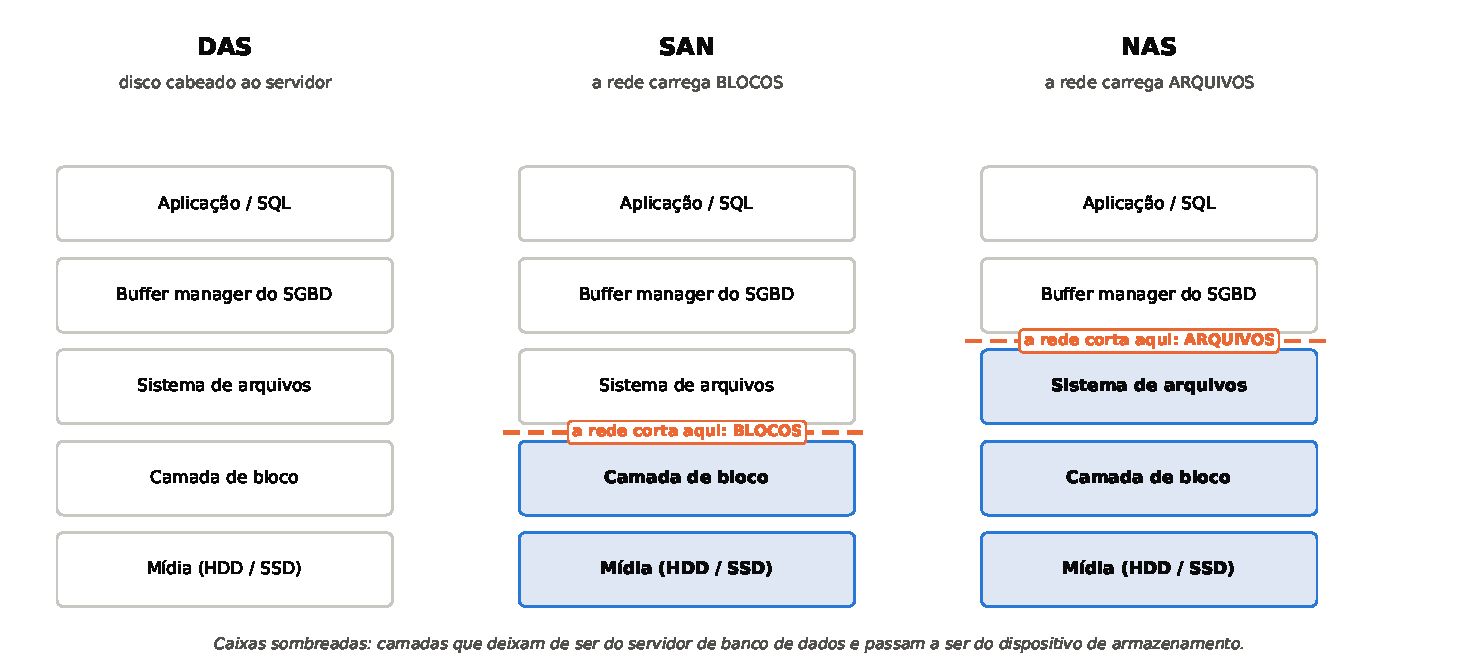
\includegraphics[width=0.80\textwidth]{fig/pilhas.pdf}
\caption{Onde a rede corta a pilha de E/S. Em SAN o corte é abaixo do sistema de arquivos (tráfego de
comandos SCSI ou NVMe); em NAS, acima (tráfego de operações de arquivo). As camadas sombreadas passam
a ser responsabilidade do dispositivo de armazenamento.}
\label{fig:pilhas}
\end{figure}

%=====================================================================
\section{NAS --- \textit{Network Attached Storage}}
\label{sec:nas}

\subsection{Como funciona}
\label{sec:nascomo}

Para Elmasri e Navathe, dispositivos NAS são servidores que ``não fornecem nenhum dos serviços comuns
de servidor'', apenas armazenamento para compartilhamento de arquivos; os clientes se conectam ao
\textit{NAS head}, e não aos discos individuais \cite{elmasri2018}. O \textit{NAS head} organiza discos
ou SSDs em RAID, monta sobre eles um sistema de arquivos próprio (WAFL na NetApp, ZFS, ext4 ou XFS) e
o exporta pela LAN via SMB/CIFS, NFS ou AFP. O servidor de banco monta o compartilhamento e emite
operações de arquivo (\textsc{open}, \textsc{read}, \textsc{write}, \textsc{lock}), não comandos de
bloco. Silberschatz resume: o NAS é ``muito parecido com SAN'', mas provê ``uma interface de sistema de
arquivos'' em vez de um disco grande \cite{silberschatz2020}.

Como alocação de blocos, \textit{journaling} e controle de concorrência ficam no dispositivo, três
consequências decorrem. \textbf{O compartilhamento é nativo}: vários servidores montam o mesmo
compartilhamento sem software extra, ao passo que dois servidores montando o mesmo LUN de uma SAN com
sistema de arquivos comum corrompem os dados, a menos que se use GFS2, OCFS2, VMFS ou gerenciador de
volume ciente de cluster. \textbf{Há independência do sistema operacional} do cliente
\cite{elmasri2018}. E \textbf{a coerência de cache é fraca por padrão}: o manual do Linux adverte que o
NFS não foi projetado para coerência de cache de sistema de arquivos de cluster, recomendando lock de
arquivo ou abertura com \texttt{O\_DIRECT} quando ela for necessária \cite{nfsman}. É por isso que os
SGBDs suportados sobre NFS usam \texttt{O\_DIRECT} ou um cliente NFS próprio.

\subsection{Protocolo NAS I --- SMB/CIFS}
\label{sec:smb}

O SMB (\textit{Server Message Block}) é o protocolo de arquivos nativo do Windows, e o CIFS não é outro
protocolo: é o nome dado ao dialeto SMB~1. A própria especificação [MS-SMB2] define o SMB~2/3 como
extensão do SMB original ``especificado em [MS-SMB] e [MS-CIFS]'' \cite{mssmb2ovw}. É um protocolo de
requisição-resposta com sessão, sobre TCP na porta 445 (historicamente NetBIOS, porta 139), com
operações de alto nível: abrir arquivo, ler ou travar intervalo de bytes, enumerar diretório.

\begin{table}[H]
\centering
\caption{Dialetos SMB relevantes. Fonte: documentação da Microsoft.}
\label{tab:smb}
{\footnotesize
\begin{tabular}{@{}L{2.1cm}L{3.6cm}L{9.0cm}@{}}
\toprule
\textbf{Dialeto} & \textbf{Introduzido em} & \textbf{O que trouxe de relevante} \\
\midrule
SMB 1.0 (CIFS) & anos 1980--1990 & Protocolo original, verboso, muitas idas e voltas por operação. \\
SMB 2.0 / 2.1 & Vista--Server 2008 / Windows 7 & Reescrita: menos comandos, requisições compostas, créditos de fluxo; \textit{leasing} de arquivo no 2.1. \\
SMB 3.0 / 3.0.2 & Windows 8--Server 2012 / 2012 R2 & SMB Direct (RDMA), \textit{Multichannel}, \textit{transparent failover}, criptografia AES-128-CCM. É a versão que torna o SMB viável para banco de dados. \\
SMB 3.1.1 & Windows 10--Server 2016 & Integridade de pré-autenticação; AES-128-GCM (AES-256-GCM a partir do Windows 11/Server 2022). \\
\bottomrule
\end{tabular}}
\end{table}

O SMBv1 não é mais instalado por padrão desde o Windows 10 Fall Creators Update e o Windows Server
versão 1709 (canal semianual), e em nenhuma edição do Windows 11 ou do Server 2019 em diante
\cite{mssmb1}. Especificar ``SMB/CIFS'' num projeto novo em 2026 significa, na prática, especificar
SMB~3.

A Microsoft suporta arquivos de banco do SQL Server (de sistema e de usuário) em compartilhamento SMB
desde o SQL Server 2012 \cite{mssqlsmb}. As condições expõem os pontos frágeis do NAS para banco: para
cargas críticas, o compartilhamento deve suportar \textit{transparent failover} do SMB~3; a conta de
serviço precisa de \textit{FULL CONTROL}; FILESTREAM não é suportado; e só valem caminhos UNC.

\subsection{Protocolo NAS II --- NFS}
\label{sec:nfs}

O NFS (\textit{Network File System}), criado pela Sun em 1984 e hoje mantido pelo IETF, é o protocolo
NAS aberto do mundo UNIX/Linux e o que efetivamente aparece em instalações de banco de dados. O NFSv2
(RFC 1094, 1989) usava UDP e \textit{offsets} de 32 bits; a Tabela~\ref{tab:nfs} traz as versões em uso.
Muita literatura ainda cita a RFC 5661 para o NFSv4.1, mas ela foi obsoletada pela RFC 8881
\cite{rfc8881}.

\begin{table}[H]
\centering
\caption{Versões do NFS em uso. ``Introduzida'' é a cronologia do protocolo; ``Norma vigente'' pode ser
reedição posterior.}
\label{tab:nfs}
{\footnotesize
\begin{tabular}{@{}L{1.3cm}L{2.3cm}L{2.3cm}L{8.8cm}@{}}
\toprule
\textbf{Versão} & \textbf{Introduzida} & \textbf{Norma vigente} & \textbf{Característica determinante} \\
\midrule
NFSv3 & 1995 & RFC 1813 & \textit{Offsets} de 64 bits, TCP, escrita assíncrona com \textit{commit} explícito. Sem estado: o lock fica num serviço à parte (NLM), o que torna frágil a recuperação após falha. \\
NFSv4.0 & 2000 (RFC 3010) & RFC 7530 (2015) & Com estado: lock, montagem e ACLs no protocolo; operações compostas; porta única 2049. \\
NFSv4.1 & 2010 (RFC 5661) & RFC 8881 (2020) & Sessões com semântica \textit{exactly-once} para requisições precedidas de \textsc{sequence} --- exigência que vale ``independentemente'' de \textit{reply caching} \cite{rfc8881}; pNFS separa metadados de dados, permitindo leitura paralela direta nos servidores de dados. \\
NFSv4.2 & 2016 & RFC 7862 & Cópia no lado do servidor, arquivos esparsos, \textit{hole punching}. \\
\bottomrule
\end{tabular}}
\end{table}

A maior limitação para banco é a consistência \textit{close-to-open}: o cliente revalida o cache ao
abrir o arquivo e descarrega alterações ao fechá-lo \cite{nfsman} --- adequado para documentos,
inadequado para um arquivo de dados que fica aberto por semanas. A Oracle resolveu isso
reimplementando o protocolo dentro do motor: o cliente \textbf{Direct NFS (dNFS)} integra a
funcionalidade de cliente NFS ao software Oracle, suporta NFSv3, NFSv4, NFSv4.1 e pNFS, e recorre ao
cliente do \textit{kernel} se não conseguir conectar \cite{oracledn}. O fato de o maior fornecedor de
bancos relacionais ter reimplementado o NAS dentro do SGBD não desqualifica o NAS; delimita a condição
em que ele funciona: quando o motor participa da decisão.

\subsection{Protocolo NAS III --- AFP (\textit{Apple Filing Protocol})}
\label{sec:afp}

O AFP é o protocolo proprietário de arquivos da Apple, nascido com o AppleTalk nos anos 1980. Sua razão
de existir era preservar as particularidades do sistema de arquivos do Macintosh --- \textit{resource
forks}, tipo e criador, nomes longos com acentuação --- que o SMB1 da época mutilava; por anos foi o
protocolo obrigatório do Time Machine em rede.

\textbf{Como funciona.} O transporte original era AppleTalk; a documentação da Apple registra que o TCP
pode ser usado ``para AFP versão 2.1 e posteriores'', na porta 548, pela camada DSI
\cite{appleafptcp}, e a partir do AFP 3.0 o AppleTalk fica restrito à descoberta de serviço. A sessão é
com estado: o cliente faz \textsc{FPLogin}, abre um volume com \textsc{FPOpenVol} e opera sobre
identificadores de sessão. Os comandos são bifurcados por \textit{fork} (\textsc{FPOpenFork},
\textsc{FPRead}/\textsc{FPWrite} sobre o \textit{data fork} ou o \textit{resource fork}), e metadados do
Finder trafegam como atributos de primeira classe. O lock por intervalo de bytes
(\textsc{FPByteRangeLock}) morre com a sessão, sem equivalente às \textit{leases} do NFSv4 ou aos
\textit{oplocks} do SMB~2/3. O AFP nunca teve caminho RDMA, \textit{multichannel} ou
\textit{failover} transparente.

\textbf{Estado atual.} O servidor AFP saiu do macOS 11 Big Sur (2020); o cliente foi depreciado no
macOS 15.5 (2025), com a Apple informando que ``será removido em uma versão futura'' \cite{appleafp};
e o Time Machine deixa de suportar destinos AFP no macOS 27 \cite{appleafptm}. A distinção cliente ×
servidor separa as duas datas por cinco anos.

\textbf{Relevância para SBD: nenhuma.} Não localizamos AFP nas matrizes de suporte de Oracle, Microsoft,
PostgreSQL e MySQL (afirmação restrita a esses quatro), e, sem lock independente de sessão nem
disponibilidade contínua, ele não atende aos requisitos 4 e 5 da Seção~\ref{sec:engine}. Para servir
clientes Apple, o caminho é o SMB, protocolo padrão de compartilhamento do macOS desde o OS X 10.9
Mavericks, que em 2013 adotou o SMB~2 no lugar do AFP \cite{appleinsider2013}. O AFP está no enunciado
como item de completude histórica, e é mais honesto dizer isso do que inventar uma aplicação de banco
para ele.

\subsection{Vantagens e desvantagens do NAS}
\label{sec:vantnas}

\begin{table}[H]
\centering
\caption{NAS sob a ótica de um SBD. As linhas de custo são \emph{estruturais}: o NAS dispensa HBA,
\textit{switch} FC e cabeamento dedicado, mas não localizamos preço público e datado que permitisse
quantificar US\$/TB, e por isso não publicamos magnitude.}
\label{tab:vantnas}
{\footnotesize
\begin{tabular}{@{}L{7.2cm}L{7.6cm}@{}}
\toprule
\textbf{Vantagens} & \textbf{Desvantagens} \\
\midrule
Usa a rede Ethernet/IP existente, sem HBA, \textit{switch} FC ou equipe especializada. & Disputa banda com a aplicação, salvo VLAN ou rede separada. \\
Compartilhamento concorrente nativo, sem sistema de arquivos de cluster. & Coerência de cache \textit{close-to-open}; exige \texttt{O\_DIRECT}, lock ou cliente dedicado \cite{nfsman}. \\
Provisionamento simples: compartilhamento e permissão, sem zoneamento nem LUN. & Camada extra de sistema de arquivos (metadados, lock, \textit{journaling}) soma latência. \\
Independência do sistema operacional do cliente \cite{elmasri2018}. & Atomicidade de página não garantida pelo protocolo; o SGBD se protege sozinho. \\
\textit{Snapshots}, clones e replicação por arquivo. & Recursos do SGBD podem faltar (FILESTREAM sobre SMB \cite{mssqlsmb}). \\
Menor custo estrutural (menos categorias de componente). & Depende de SMB~3 \textit{transparent failover} ou sessões NFSv4.1 para sobreviver a falhas. \\
\bottomrule
\end{tabular}}
\end{table}
%=====================================================================
\section{SAN --- \textit{Storage Area Network}}
\label{sec:san}

\subsection{Como funciona}
\label{sec:sancomo}

Na definição de Silberschatz, na SAN ``um grande número de discos é conectado por uma rede de alta
velocidade a um conjunto de computadores servidores'', organizados em RAID para oferecer ``uma visão
lógica de um disco muito grande e muito confiável'' \cite{silberschatz2020}. A sequência operacional,
em contraste com o NAS, é: (1) o \textit{array} agrega discos em \textit{pools} protegidos por RAID ou
codificação de apagamento; (2) o administrador recorta volumes e os apresenta como \textbf{LUNs}
(\textit{Logical Unit Numbers}); (3) uma rede dedicada (FC ou Ethernet segregada) transporta comandos
SCSI --- ou NVMe --- entre o iniciador no servidor e o alvo no \textit{array}; (4) o sistema operacional
enxerga um dispositivo de bloco cru, indistinguível de um disco local, e o formata ou o entrega cru ao
SGBD (como faz o Oracle ASM). Elmasri e Navathe capturam o efeito: as redes \textit{Fibre Channel}
encapsulam o SCSI legado, e por isso os dispositivos da SAN ``aparecem como dispositivos SCSI''
\cite{elmasri2018}. O servidor e o SGBD não precisam saber que há uma rede no caminho.

\subsection{\textit{Fibre Channel}: a pilha}
\label{sec:fc}

O \textit{Fibre Channel} é padronizado pelo comitê T11 do INCITS. A grafia normativa é
\textit{Fibre}, justamente porque o padrão não exige fibra óptica; os livros da disciplina alternam com
``\textit{Fiber}'' \cite{elmasri2018,silberschatz2020}.

\begin{table}[H]
\centering
\caption{Camadas do \textit{Fibre Channel} (arquitetura T11/INCITS).}
\label{tab:fcpilha}
{\footnotesize
\begin{tabular}{@{}L{1.3cm}L{2.2cm}L{11.3cm}@{}}
\toprule
\textbf{Camada} & \textbf{Nome} & \textbf{Função} \\
\midrule
FC-0 & Físico & Meio, conectores, transceptores, taxa de sinalização. \\
FC-1 & Codificação & 8b/10b até 8GFC; 64b/66b no 16GFC; 256b/257b com RS-FEC a partir de 32GFC; PAM-4 a partir de 64GFC. \\
FC-2 & Sinalização & Quadros, sequências, trocas (\textit{exchanges}) e controle de fluxo por créditos (BB\_Credit). \\
FC-3 & Serviços comuns & Serviços entre múltiplas portas (\textit{hunt groups}, \textit{striping}); pouco usada. \\
FC-4 & Mapeamento & Protocolos superiores sobre FC: FCP (SCSI-3 sobre FC) e, mais recentemente, FC-NVMe. \\
\bottomrule
\end{tabular}}
\end{table}

\textbf{Controle de fluxo por créditos.} Diferentemente do Ethernet clássico, que descarta quadros sob
congestionamento e deixa a recuperação ao TCP, no FC-2 uma porta só transmite se tiver crédito, e o
crédito volta quando o vizinho libera um \textit{buffer}. A rede é sem perdas por congestionamento, o
que permite dispensar o TCP. O custo é que, quando os créditos acabam, o enlace \emph{para}: um
dispositivo lento pode congelar tráfego alheio que compartilhe o caminho (\textit{slow drain}).

\textbf{Dimensionamento (derivação nossa):} a luz em fibra leva $\approx$5 µs/km, e os 10 km que Elmasri e
Navathe citam como alcance da SAN \cite{elmasri2018} somam 50 µs por sentido. A 32GFC (3.200 MB/s por
direção), ficam $50 \times 10^{-6}\,\text{s} \times 3{,}2 \times 10^{9}\,\text{B/s} = 160$ kB em trânsito, ou
$\approx$76 quadros de 2.112 bytes; com o retorno do crédito, $\approx$150 BB\_Credits mantêm o enlace cheio. O
\textit{switch} Brocade G710 declara 2.000 \textit{buffers} de quadro alocados dinamicamente \cite{brocadeg710},
uma ordem de grandeza acima, o que permite enlaces bem mais longos sem ociosidade por falta de crédito.

\textbf{Endereçamento e zoneamento.} Cada porta tem um WWN de 64 bits gravado de fábrica; ao entrar na
\textit{fabric} (\textsc{flogi}) recebe um endereço de 24 bits usado no roteamento. O
\textbf{zoneamento}, no \textit{switch}, define quais iniciadores veem quais alvos; o \textbf{LUN
masking}, no \textit{array}, define quais LUNs cada iniciador enxerga. Juntos, impedem que o servidor de
teste monte o LUN de produção.

\textbf{Velocidades e rótulos.} A Tabela~\ref{tab:speedmap} reproduz o \textit{speedmap} vigente da
FCIA para FC serial \cite{fciaroadmap}. Os valores da FCIA são a \emph{soma dos dois sentidos}: o
\textit{speedmap} não o declara, mas o \textit{webcast} técnico da própria FCIA sobre o 128GFC publica a
escala por direção --- 6.400 MB/s para o 64GFC e 12.425 MB/s para o 128GFC \cite{fcia128webcast} ---, e
a física confirma: os 3.200 MB/s do 16GFC equivalem a 25,6 Gb/s, mais do que a linha comporta num sentido --- 14,025 GBd em NRZ, isto é, 14,025 Gb/s brutos, já que NRZ transmite 1 bit por símbolo. Para
dimensionar o caminho de E/S de um SGBD, vale a coluna ``por direção''.

\begin{table}[H]
\centering
\caption{\textit{Speedmap} FC serial (FCIA v24, jul./2023) \cite{fciaroadmap}. ``Por direção'' é metade do
valor da FCIA, escala confirmada em \cite{fcia128webcast}. ``Gb/s brutos'' $=$ GBd $\times$ bits por símbolo (1 em
NRZ, 2 em PAM-4), conversão nossa.}
\label{tab:speedmap}
{\footnotesize
\begin{tabular}{@{}lrrlrcc@{}}
\toprule
\textbf{Produto} & \textbf{\makecell[r]{FCIA\\(MB/s)}} & \textbf{\makecell[r]{Por direção\\(MB/s)}} & \textbf{\makecell[l]{Linha\\(GBd)}} & \textbf{\makecell[r]{Gb/s\\brutos}} & \textbf{\makecell{Norma\\T11}} & \textbf{Mercado} \\
\midrule
8GFC & 1.600 & 800 & 8,5 NRZ & 8,5 & 2006 & 2008 \\
16GFC & 3.200 & 1.600 & 14,025 NRZ & 14,025 & 2009 & 2011 \\
32GFC & 6.400 & 3.200 & 28,05 NRZ & 28,05 & 2013 & 2016 \\
64GFC & 12.800 & 6.400 & 28,9 PAM-4 & 57,8 & 2017 & 2020 \\
128GFC & 24.850 & 12.425 & 56,1 PAM-4 & 112,2 & 2022 & 2024 \\
256GFC & 49.700 & 24.850 & 112,2 PAM-4 & 224,4 & 2025 & demanda \\
\bottomrule
\end{tabular}}
\end{table}

\destaque{Achado de rótulo: três números atendem por ``128GFC''}{%
Até o 64GFC vale a convenção ``$X$GFC $=$ $X \times 100$ MB/s por direção''. No 128GFC ela quebra: dobrar a
velocidade exigiria linha de 115,6 Gb/s, e a FCIA registra que o \textit{link budget} não fechava
\cite{fcia128}; a linha ficou em 56,1 GBd em PAM-4, isto é, 112,2 Gb/s brutos, e a vazão por direção é 12.425
MB/s, não 12.800 (a eficiência útil, $99{,}4 / 112{,}2 = 88{,}6\%$, é a mesma do 64GFC, $51{,}2 / 57{,}8$). Resultado:
\textbf{25.600 MB/s} é o 128GFC de \textit{Inter-Switch Link} (4 vias de 28,05 GBd, 2016); \textbf{24.850
MB/s} é o 128GFC serial (Gen 8, 2024); e \textbf{12.800 MB/s} é o valor que a FC-PI-8 mantém como
\textit{Data Rate}, deliberadamente não atualizado \cite{fcia128}. Citar ``128GFC'' sem dizer qual erra por
até $2\times$.}

O mesmo cuidado vale para o Silberschatz, que informa ``de 1,6 a 12 gigabytes por segundo, dependendo da
versão'' \cite{silberschatz2020}: 1,6 GB/s é o 16GFC por direção, e $\approx$12 GB/s corresponde aos 12.800
MB/s do 64GFC somados nos dois sentidos. A faixa é compatível com as gerações da época, mas mistura as duas
escalas sem declarar; registramos como ambiguidade de rótulo, e não como erro.

\subsection{Topologias FC --- o ``FC \textit{Switch}'' do enunciado}
\label{sec:topologias}

``FC \textit{Switch}'' não é um protocolo, e sim uma das três topologias definidas pelo T11, que Elmasri e
Navathe apresentam como alternativas arquiteturais para SAN \cite{elmasri2018}.

\begin{table}[H]
\centering
\caption{Topologias \textit{Fibre Channel}.}
\label{tab:topologias}
{\footnotesize
\begin{tabular}{@{}L{3.0cm}L{11.8cm}@{}}
\toprule
\textbf{Topologia} & \textbf{Descrição e situação atual} \\
\midrule
Ponto-a-ponto (FC-P2P) & Dois dispositivos ligados diretamente, sem \textit{switch}; banda dedicada, dois nós. Uso residual (servidor ligado direto ao \textit{array}). \\
\textit{Arbitrated loop} (FC-AL) & Anel com até 126 NL\_Ports mais uma FL\_Port (127 endereços) e banda compartilhada; a inserção de um nó reinicializa o anel (LIP) e pausa a E/S. Obsoleta. \\
\textit{Switched fabric} (FC-SW) & \textbf{O ``FC \textit{Switch}'' do enunciado} e a topologia de toda SAN FC moderna: banda dedicada por porta, roteamento FSPF, zoneamento, endereçamento de 24 bits, \textit{switches} ligados por ISLs agregáveis em \textit{trunks}. Prática padrão: duas \textit{fabrics} independentes (``SAN A'' e ``SAN B''), com uma HBA do servidor em cada. \\
\bottomrule
\end{tabular}}
\end{table}

\textbf{Ordem de grandeza da latência.} O \textit{switch} Brocade G710 (64GFC) declara 460 ns para
portas comutadas localmente, incluindo FEC \cite{brocadeg710}. Dois saltos somam menos de 1 µs, menos de
5\% de uma leitura aleatória em SSD, que Silberschatz situa entre 20 e 100 µs \cite{silberschatz2020}
(derivação nossa). A conta isola a comutação; não inclui HBA, filas, ISLs, controladora nem alvo, e
portanto não prova que a rede fim a fim deixou de importar.

\subsection{Protocolo SAN I --- FCP sobre \textit{Fibre Channel}}
\label{sec:fcp}

O FCP é o mapeamento FC-4 que transporta comandos, dados e respostas SCSI-3 em quadros FC. Cada operação
é uma troca iniciada pelo iniciador e encerrada pelo alvo:

\begin{center}\footnotesize
\textbf{Leitura:} \texttt{FCP\_CMND} \seta\ \texttt{FCP\_DATA} \seta\ \texttt{FCP\_RSP}
\qquad
\textbf{Escrita:} \texttt{FCP\_CMND} \seta\ \texttt{FCP\_XFER\_RDY} \seta\ \texttt{FCP\_DATA} \seta\ \texttt{FCP\_RSP}
\end{center}

O \texttt{FCP\_CMND} leva o CDB SCSI e o LUN; o \texttt{FCP\_DATA} leva a carga útil em quantos quadros
forem necessários (até 2.112 bytes por quadro); o \texttt{FCP\_RSP} devolve o status. Na escrita, o
\texttt{FCP\_XFER\_RDY} é o alvo informando quanto está pronto para receber --- uma ida e volta a mais,
que pesa diretamente na latência de \texttt{fsync} do \textit{log} (Seção~\ref{sec:engine}). Esse
controle opera por comando (FC-4) e é independente do BB\_Credit, que opera por quadro (FC-2).
Características determinantes do FCP: rede sem perdas que dispensa TCP; rede fisicamente separada da
aplicação, o que simplifica o diagnóstico; pilha inteira processada na HBA; e, em contrapartida, custo
de HBAs, \textit{switches} e cabeamento dedicados, além de equipe que domine zoneamento e
\textit{fabrics} redundantes.

\subsection{Protocolo SAN II --- iSCSI}
\label{sec:iscsi}

O iSCSI encapsula comandos SCSI em TCP/IP, permitindo uma SAN de bloco sobre Ethernet comum. A norma
vigente é a RFC 7143 (2014), que obsoletou a RFC 3720 ainda citada em boa parte do material didático
\cite{rfc7143}. Elmasri e Navathe descrevem o fluxo: o sistema operacional gera os comandos SCSI, que
são encapsulados (e, se necessário, criptografados) em pacotes IP e transmitidos por Ethernet
\cite{elmasri2018}. Iniciador e alvo são identificados por IQN (por exemplo,
\texttt{iqn.2026-09.br.ufrj.dcc:servidor01}); o transporte é TCP na porta 3260; a autenticação, CHAP; a
confidencialidade, IPsec opcional; e a descoberta, \textsc{SendTargets} ou iSNS.

Três mecanismos o distinguem do FCP. O \textbf{R2T} é o equivalente do \texttt{XFER\_RDY}, e as opções
\textit{ImmediateData} e \textit{InitialR2T=No}, negociadas no \textit{login}, poupam uma ida e volta por
escrita. Os \textbf{digests} CRC-32C de cabeçalho e dados são opcionais (o TCP tem só um
\textit{checksum} de 16 bits) e custam CPU. E \textbf{MC/S × MPIO}: o primeiro agrega conexões TCP numa
sessão; o segundo agrega sessões no \textit{host} e é o recomendado, porque integra com ALUA e com o
\textit{failover} do sistema operacional.

A vantagem, segundo Elmasri e Navathe, é dispensar o cabeamento especial do FC e operar a distâncias
maiores sobre a infraestrutura existente; por isso o iSCSI se consolidou em empresas de pequeno e médio
porte, enquanto grandes \textit{data centers} demoraram a adotá-lo pelo investimento prévio em FC
\cite{elmasri2018}. A desvantagem é a pilha TCP/IP (CPU do \textit{host}, perdas sob congestionamento),
mitigada hoje por TOE ou HBA iSCSI, por iSER (RDMA) e por DCB no \textit{switch}.

\subsection{Protocolo SAN III --- FCIP}
\label{sec:fcip}

O FCIP (RFC 3821, 2004, vigente e atualizada pela RFC 7146 quanto a IPsec v3 \cite{rfc3821,rfc7146}) não
substitui o FC: é um \textbf{túnel} que, nas palavras de Elmasri e Navathe, traduz controle e dados FC em
pacotes IP entre SANs FC geograficamente distantes e ``só pode ser usado em conjunto com tecnologia
\textit{Fibre Channel}'' \cite{elmasri2018}. A distinção com o iSCSI é conceitual: \textbf{o iSCSI
substitui o FC} (não há HBA FC nem \textit{fabric}), enquanto \textbf{o FCIP preserva o FC} (as duas
pontas são \textit{fabrics} completas, com WWNs e zoneamento). Sem isolamento, a extensão pode unir as
\textit{fabrics} e propagar reconfigurações entre sítios, por isso os produtos oferecem FC
\textit{routing}/IVR.

A aplicação típica é replicação entre sítios para recuperação de desastre \cite{elmasri2018}, e a física
decide o modo. Com luz em fibra a $\approx 2 \times 10^{8}$ m/s, a ida e volta custa
$t_{RTT} = 2d / (2 \times 10^{8}\ \text{m/s}) = 1$ ms a cada 100 km, só de propagação (derivação nossa).
Para um \textit{commit} local de $\approx$100 µs, replicar sincronamente a 100 km multiplica a latência
por mais de dez; por isso a replicação síncrona fica restrita a campus e área metropolitana, e a
intercontinental é tipicamente assíncrona, com RPO maior que zero.

\subsection{Protocolo SAN IV --- FCoE}
\label{sec:fcoe}

O FCoE encapsula quadros FC inteiros diretamente em quadros Ethernet, sem TCP e sem IP. Foi padronizado
no FC-BB-5 (ANSI/INCITS 462-2010), e o FC-BB-6 acrescentou o modo VN2VN, sem \textit{switch} FCF
\cite{fcbb5}. Elmasri e Navathe o descrevem como algo que ``pode ser pensado como iSCSI sem o IP'', mas o
mesmo parágrafo qualifica a analogia: não inclui TCP/IP e depende de uma Ethernet confiável com
\textit{buffering} e controle de fluxo \cite{elmasri2018}.

Restam duas imprecisões reais. \textbf{O controle de fluxo não é fim a fim, e sim enlace a enlace}: o PFC
(IEEE 802.1Qbb) pausa por prioridade entre vizinhos adjacentes \cite{ieee8021qbb}, e é isso que produz o
\textit{congestion spreading}, em que um alvo lento propaga pausas e degrada tráfego não relacionado.
\textbf{O FCoE não é roteável em camada 3}: usa \textit{EtherTypes} próprios (0x8906 para dados, 0x8914
para o FIP), sem cabeçalho IP, e vive dentro de um domínio de camada 2 (análise nossa apoiada no
encapsulamento definido pela norma). Quem ler ``iSCSI sem o IP'' e tentar ligar dois \textit{data
centers} com FCoE não conseguirá; para a WAN, os caminhos são FCIP ou iSCSI. A promessa do FCoE era a
convergência (um par de CNAs para LAN e SAN), e ele foi produtizado por Cisco e Brocade
\cite{elmasri2018}; na prática, prevaleceu dentro do \textit{rack} (\textit{blades}, sistemas
convergentes) e ocupa um nicho entre o FC e o iSCSI.

\subsection{Multipath e RAID: o que a SAN pressupõe}
\label{sec:multipath}

O requisito 5 (Seção~\ref{sec:engine}) não é atendido pelo protocolo, e sim por arquitetura. Duas
\textit{fabrics} só produzem disponibilidade se o \textit{host} reconhecer que os caminhos levam ao
mesmo LUN (DM-Multipath no Linux, MPIO no Windows), com ALUA indicando os caminhos otimizados em
\textit{arrays} assimétricos. O que torna uma falha de caminho invisível ou fatal ao SGBD é a
configuração de \texttt{no\_path\_retry} e \texttt{fast\_io\_fail\_tmo}: enfileirar indefinidamente
congela a instância; falhar imediatamente aborta transações. É decisão de projeto, não padrão a aceitar.

Quanto ao RAID, Silberschatz observa que uma escrita aleatória no nível 5 exige ``2 leituras de bloco
\ldots\ e 2 escritas de bloco'', e que o nível 1 é popular para arquivos de \textit{log} por oferecer o
melhor desempenho de escrita \cite{silberschatz2020}. Em operações físicas por escrita aleatória: RAID 1
$= 2$, RAID 5 $= 4$, RAID 6 $= 6$. Daí a regra prática: \textit{log} em RAID 1/10, dados em RAID 5/6 --- e
volume de \textit{redo} com política de \textit{tiering} fixada (Seção~\ref{sec:ast}).

\subsection{Vantagens e desvantagens da SAN}
\label{sec:vantsan}

\begin{table}[H]
\centering
\caption{SAN sob a ótica de um SBD.}
\label{tab:vantsan}
{\footnotesize
\begin{tabular}{@{}L{7.2cm}L{7.6cm}@{}}
\toprule
\textbf{Vantagens} & \textbf{Desvantagens} \\
\midrule
Semântica de bloco cru: o SGBD controla alocação, cache e ordem de escrita. & Custo de HBAs, \textit{switches}, transceptores, cabeamento e duas \textit{fabrics}. \\
Rede dedicada, sem interferência da aplicação. & Exige competência em zoneamento, LUN \textit{masking}, \textit{multipath} e diagnóstico de \textit{fabric}. \\
Conectividade flexível muitos-para-muitos entre servidores e armazenamento \cite{elmasri2018}. & Compartilhar LUN exige sistema de arquivos ou LVM ciente de cluster. \\
Até 10 km entre servidor e armazenamento com fibra adequada \cite{elmasri2018}; além disso, FCIP. & SCSI legado herda modelo de fila pensado para disco mecânico (daí o NVMe-oF). \\
Adição não disruptiva de periféricos e servidores \cite{elmasri2018}. & Integrar vários fornecedores e padrões em evolução continua difícil \cite{elmasri2018}. \\
Comutação local pequena diante da latência da mídia (Seção~\ref{sec:topologias}). & Um erro de zoneamento pode tornar o dado inacessível a todos os servidores. \\
\bottomrule
\end{tabular}}
\end{table}

%=====================================================================
\section{Quadro comparativo consolidado}
\label{sec:comparativo}

A confusão entre iSCSI, FCIP e FCoE desaparece quando se vê o que cada protocolo coloca dentro de quê
(Figura~\ref{fig:encaps}): iSCSI e FCoE não são variantes um do outro; FCIP e FCoE carregam o mesmo
quadro FC sobre meios diferentes, e por isso um é roteável e o outro não; e o NAS é o único cuja unidade
não é o bloco.

\begin{figure}[H]
\centering
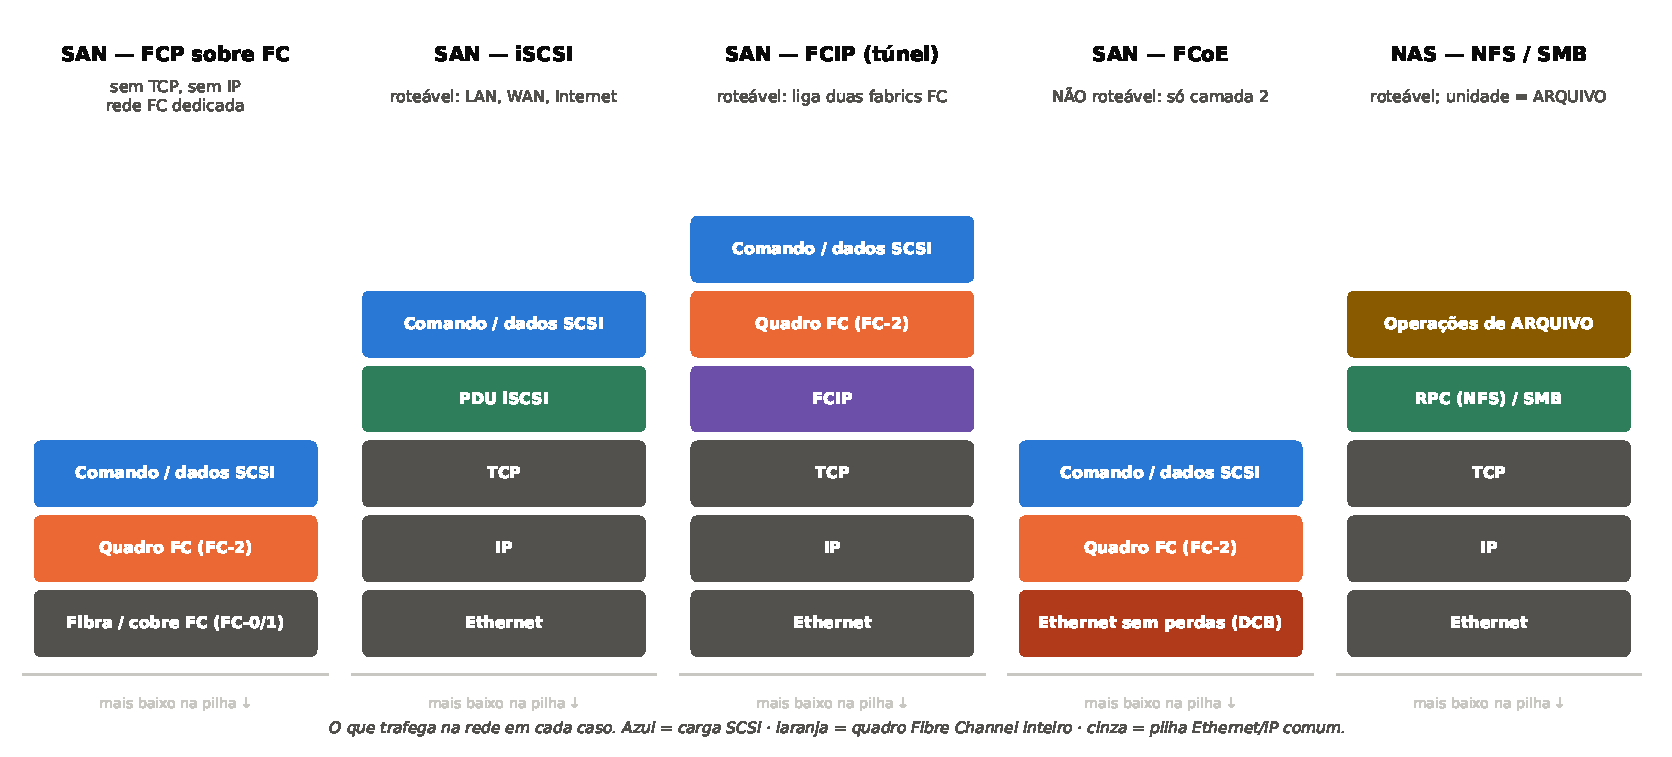
\includegraphics[width=\textwidth]{fig/encapsulamento.pdf}
\caption{O que trafega na rede em cada arquitetura. Azul: carga SCSI; laranja: quadro FC inteiro;
cinza: pilha Ethernet/IP.}
\label{fig:encaps}
\end{figure}

\begin{table}[H]
\centering
\caption{Protocolos exigidos pelo enunciado, com norma e propriedades decisivas.}
\label{tab:protocolos}
{\scriptsize \setlength{\tabcolsep}{3pt}
\begin{tabular}{@{}>{\RaggedRight\arraybackslash}L{1.55cm}
                >{\RaggedRight\arraybackslash}p{0.75cm}
                >{\RaggedRight\arraybackslash}p{3.0cm}
                >{\RaggedRight\arraybackslash}p{2.9cm}
                >{\RaggedRight\arraybackslash}p{1.4cm}
                >{\RaggedRight\arraybackslash}p{5.15cm}@{}}
\toprule
\textbf{Protocolo} & \textbf{Fam.} & \textbf{Norma / origem} & \textbf{Unidade e transporte} & \textbf{Roteável L3?} & \textbf{Estado e uso em SGBD (2026)} \\
\midrule
SMB/CIFS & NAS & [MS-SMB2]; CIFS $=$ SMB~1 \cite{mssmb2ovw} & Operações de arquivo; TCP 445 & Sim & SMB 3.1.1 corrente; SMB~1 fora por padrão \cite{mssmb1}. SQL Server suportado com \textit{transparent failover} \cite{mssqlsmb}. \\
NFS & NAS & IETF: RFCs 1813, 7530, 8881, 7862 & Operações de arquivo (RPC); TCP 2049 (v4) & Sim & Suportado com cliente dedicado (Oracle dNFS) ou \texttt{O\_DIRECT} \cite{oracledn}. \\
AFP & NAS & Proprietário Apple & Operações de arquivo; TCP 548 (DSI) & Sim & Em fim de vida \cite{appleafp,appleafptm}; sem uso em SGBD. \\
FCP sobre FC & SAN & T11/INCITS; FCP $=$ SCSI-3 em FC-4 & Comandos SCSI em quadros FC; rede sem perdas & Não & Referência para OLTP crítico e RAC/ASM; 64GFC corrente, 128GFC em implantação. \\
FC \textit{Switch} (FC-SW) & SAN & T11 --- topologia, não protocolo & Transporta FCP; roteamento FSPF & Não & Topologia padrão da SAN FC, com duas \textit{fabrics}. \\
iSCSI & SAN & RFC 7143, obsoleta a 3720 \cite{rfc7143} & Comandos SCSI em TCP 3260 & Sim & Consolidado em pequeno e médio porte; bloco com custo menor. \\
FCIP & SAN & RFC 3821, atualizada pela 7146 \cite{rfc3821,rfc7146} & Quadros FC inteiros em TCP/IP & Sim & Túnel entre \textit{fabrics}; replicação para DR. \\
FCoE & SAN & FC-BB-5 (INCITS 462-2010); FC-BB-6 \cite{fcbb5} & Quadros FC em Ethernet sem perdas (DCB) & Não & Nicho: convergência dentro do \textit{rack}. \\
NVMe-oF & SAN & NVM Express & Comandos NVMe sobre FC, TCP ou RDMA & Depende & Em adoção; substitui o SCSI, não o meio (nota de fronteira). \\
\bottomrule
\end{tabular}}
\end{table}

\begin{table}[H]
\centering
\caption{NAS × SAN: as dimensões que decidem a escolha.}
\label{tab:nasxsan}
{\footnotesize
\begin{tabular}{@{}L{3.3cm}L{5.6cm}L{5.9cm}@{}}
\toprule
\textbf{Dimensão} & \textbf{NAS} & \textbf{SAN} \\
\midrule
Unidade de abstração & Arquivo & Bloco (LUN) \\
Dono do sistema de arquivos & Dispositivo de armazenamento & Servidor \\
Protocolos & SMB/CIFS, NFS, AFP & FCP/FC, iSCSI, FCIP, FCoE \\
Compartilhamento & Nativo; o dispositivo arbitra & Exige sistema de arquivos ou LVM de cluster \\
Lock & No protocolo (NLM no NFSv3; integrado no NFSv4; \textit{leases} no SMB) & No servidor; a SAN não sabe o que é arquivo \\
Coerência de cache & Depende do protocolo; NFS usa \textit{close-to-open} \cite{nfsman} & Coordenada pelos servidores \\
Distância & Rede IP; latência limita a aplicação & Óptica e transporte; FCIP não elimina latência \\
Uso típico em SBD & \textit{Backup}, análise e bancos em configurações NFS/SMB homologadas & OLTP crítico, clusters compartilhados, requisito de latência de \textit{commit} \\
\bottomrule
\end{tabular}}
\end{table}

Os próprios livros já anunciavam a convergência: Silberschatz registra que sistemas SAN e NAS modernos
combinam discos e SSDs, usando os SSDs como cache \cite{silberschatz2020}. Em 2026, quase todo
\textit{array} corporativo é unificado --- apresenta LUNs por FC ou iSCSI e compartilhamentos por NFS e
SMB sobre o mesmo \textit{pool}. A pergunta ``comprar NAS ou SAN?'' virou ``qual protocolo apresentar
para cada carga?'', que admite respostas diferentes para o \textit{tablespace} e para a área de
\textit{dump}.
%=====================================================================
\section{AST --- \textit{Automated Storage Tiering}}
\label{sec:ast}

\subsection{O que é e como funciona}

Elmasri e Navathe definem o AST como a técnica que ``move automaticamente dados entre diferentes tipos de
armazenamento, como SATA, SAS e \textit{solid-state drives}'', segundo uma política em que dados pouco
usados vão para discos lentos e baratos e dados frequentes vão para SSD; citam como referência o FAST da
EMC, que monitora continuamente a atividade e move os dados para o \textit{tier} apropriado
\cite{elmasri2018}. A técnica existe porque a hierarquia de armazenamento ordena os meios por preço por
byte e o acesso a dados é enviesado: uma fração pequena dos blocos concentra a maioria dos acessos, e
comprar flash para o banco inteiro é pagar pelo pior caso em toda a capacidade.

Como exemplo documentado, o Dell EMC Unity FAST VP \cite{dellfast} espalha os dados de um \textit{pool}
multicamada em \textbf{fatias de 256 MB} entre três \textit{tiers} (flash; SAS 10K/15K; NL-SAS 7,2K);
\textbf{uma vez por hora} classifica cada fatia pela sua ``temperatura'' de acesso; e move fisicamente as
fatias numa \textbf{janela agendada e configurável}. As políticas são \textit{Highest Available Tier},
\textit{Auto-Tier}, \textit{Lowest Available Tier} e \textit{Start High then Auto-Tier}, esta a recomendada
como padrão.

\subsection{AST e \textit{buffer pool}}
\label{sec:asttensao}

O \textit{buffer manager} do SGBD, a que Elmasri e Navathe dedicam a Seção 16.3.1, também decide o que
fica na camada rápida, mas de modo muito diferente. \textbf{Granularidade:} ele decide por página, o AST
por fatia; lendo os 256 MB como 256 MiB, a razão é $256\ \text{MiB} / 16\ \text{KiB} = 16.384\times$
(InnoDB) ou $32.768\times$ para páginas de 8 KiB (derivação nossa) --- se 1 MB da fatia estiver quente e
255 MB frios, o AST promove os 256 MB. \textbf{Reação:} o \textit{buffer manager} reage ao acesso; o AST,
numa janela de horas. \textbf{Semântica:} o \textit{buffer manager} sabe que a página é a raiz de um
índice B$^+$; o \textit{array} vê apenas endereços de bloco. Três consequências práticas:

\begin{enumerate}[leftmargin=0.7cm,itemsep=1pt]
\item \textbf{O AST vê a carga filtrada pelo \textit{buffer pool}.} Um bloco muito quente que mora em
memória quase nunca é relido do disco e pode ser classificado como frio --- justamente o dado mais quente
do banco.
\item \textbf{Conjuntos quentes móveis derrotam o AST.} Com particionamento por data, a partição quente
muda mais rápido que a janela de relocação. A política \textit{Start High then Auto-Tier} mitiga isso
gravando tudo no \textit{tier} rápido e só depois esfriando o que não é acessado \cite{dellfast}.
\item \textbf{Cache e \textit{tiering} são mecanismos diferentes.} Cache mantém uma \emph{cópia} na camada
rápida; AST \emph{migra} a localização. Um não substitui automaticamente o outro em OLTP.
\end{enumerate}

\subsection{Recomendação sobre AST}
\label{sec:astrec}

\begin{itemize}[leftmargin=0.7cm,itemsep=1pt]
\item \textbf{Habilitar} em \textit{data warehouses} com grande volume histórico frio e na consolidação de
muitos bancos pequenos num \textit{pool} comum: o padrão de acesso é estável na escala de dias.
\item \textbf{Evitar, ou fixar em \textit{Highest Available Tier}}, \textit{redo}/WAL, \textit{tempdb} e
índices críticos, cujo desempenho não pode depender de decisão estatística tomada horas depois.
\item \textbf{Nunca usar AST como substituto de dimensionamento}: se o conjunto quente não cabe no
\textit{tier} rápido, o AST só redistribui a escassez e acrescenta tráfego de migração.
\item \textbf{Não confundir com proteção de dados}: AST otimiza posicionamento, não cria cópia
recuperável; \textit{backup} e replicação continuam necessários.
\end{itemize}

%=====================================================================
\section{\textit{Object-Based Storage}}
\label{sec:objeto}

\subsection{O terceiro paradigma}

Elmasri e Navathe descrevem o armazenamento por objetos: os dados são geridos como objetos, e não como
arquivos feitos de blocos; cada objeto carrega metadados usados para gerenciá-lo e ``um identificador
global único'' usado para localizá-lo \cite{elmasri2018}. A Tabela~\ref{tab:paradigmas} contrasta os três
paradigmas.

\begin{table}[H]
\centering
\caption{Os três paradigmas de armazenamento em rede.}
\label{tab:paradigmas}
{\footnotesize
\begin{tabular}{@{}L{2.6cm}L{3.6cm}L{3.8cm}L{4.6cm}@{}}
\toprule
 & \textbf{Bloco (SAN)} & \textbf{Arquivo (NAS)} & \textbf{Objeto} \\
\midrule
Endereçamento & LUN $+$ LBA & Caminho hierárquico & Espaço plano (\textit{bucket} $+$ chave) \\
Interface & SCSI / NVMe & POSIX, SMB, NFS & HTTP REST (\textsc{put}, \textsc{get}, \textsc{delete}) \\
Atualização parcial & Qualquer bloco & Qualquer \textit{offset} & Não: \textsc{put} substitui o objeto \\
Metadados & Nenhum & Fixos (dono, datas, permissões) & Arbitrários, da aplicação \\
Consistência e lock & Definidos pelo \textit{host}/SGBD & Locks/\textit{leases} conforme versão & Forte por chave e listagem no S3; sem transação entre chaves \cite{awss3consistency} \\
Escala típica & TB a PB & TB a PB & Até exabytes \\
Melhor uso & OLTP, \textit{logs}, clusters & Compartilhamento, DW, \textit{dumps} & \textit{Data lake}, \textit{backup}, arquivo \\
Exemplos & LUN FC/iSCSI/NVMe-oF & NFSv4.1, SMB 3 & Amazon S3, Ceph RGW, MinIO \\
\bottomrule
\end{tabular}}
\end{table}

\subsection{Origem e o que prevaleceu}

Elmasri e Navathe situam a origem nos projetos da CMU sobre \textit{network attached storage} (Gibson
\textit{et al.}, 1996) e no OceanStore de Berkeley (Kubiatowicz \textit{et al.}, 2000), e registram que os
comandos OSD propostos no SCSI só viraram produto com a plataforma Kinetic da Seagate \cite{elmasri2018}.
A ideia central do NASD de 1996 foi separar o plano de controle (metadados, autorização) do plano de
dados, a mesma que reaparece no pNFS (Seção~\ref{sec:nfs}) e no NDMP (Seção~\ref{sec:recterciario}).

A Kinetic não obteve tração comercial: a cobertura de 2016 relata que a HGST passou um ano procurando
casos de uso com clientes sem encontrar nenhum \cite{theregister2016}. Não localizamos anúncio formal de
descontinuação, por isso não afirmamos que ela foi descontinuada. O que prevaleceu foi a interface HTTP ---
o próprio livro já aponta S3, Azure e o \textsc{get}/\textsc{put} do OpenStack Swift \cite{elmasri2018}; a
nossa leitura, sem fonte que a quantifique, é que a API do S3 virou a interface que os demais implementam
por compatibilidade.

\subsection{Propriedades e limites para SGBD}

O armazenamento por objetos troca recursos por escala: abre mão da hierarquia (o espaço plano é
particionável por \textit{hash} sem coordenação central), da atualização parcial (objetos imutáveis
simplificam replicação e versionamento) e do POSIX (sem \texttt{fsync}, lock de intervalo ou
\textit{rename} atômico). Em troca, obtém durabilidade por codificação de apagamento: a AWS declara o S3
``projetado para'' 11 noves de durabilidade \cite{awss3faq} --- objetivo de projeto, não SLA, e por isso
não o convertemos em ``anos até uma perda''. Desde dezembro de 2020 o S3 oferece consistência forte
\textit{read-after-write}, inclusive em listagens \cite{awss3news2020,awss3consistency}; a garantia é por objeto, não uma
transação entre chaves.

Por isso uma API de objetos não substitui diretamente o dispositivo de blocos de um motor OLTP
tradicional: não há atualização de página \textit{in place}, nem \texttt{fsync}, nem ordenação de escrita
entre objetos, e o motor teria de implementar ordenação de \textit{log}, concorrência e recuperação. O
objeto é adequado como camada de armazenamento de \textit{data warehouses} em nuvem (arquivos colunares
com camada transacional de metadados), destino de \textit{backup} e arquivamento, e repositório de dados
não estruturados --- Elmasri e Navathe citam Facebook, Spotify e Dropbox \cite{elmasri2018}.

%=====================================================================
\section{Recomendação geral}
\label{sec:recomendacao}

\destaque{A regra de decisão}{%
\textbf{Escolha pela semântica oficialmente suportada pelo SGBD e pelo SLA, não pela velocidade do
enlace.} Bloco (SAN) é o padrão em OLTP crítico e clusters com armazenamento compartilhado, mas NFS e SMB
homologados (dNFS, SMB~3 com \textit{transparent failover}) também entregam durabilidade, lock e
\textit{failover} adequados. Compare protocolo e cliente, latência de cauda (P99), comportamento sob
falha, RPO/RTO e TCO medidos na configuração real. Objeto só quando a aplicação foi projetada para sua
API.}

\subsection{Nível secundário (\textit{storage online})}
\label{sec:recsecundario}

É onde vivem arquivos de dados, índices e \textit{log} de transações --- tudo que o motor acessa em
execução normal. A recomendação é por perfil de carga, não por porte de empresa.

\begin{table}[H]
\centering
\caption{Recomendação para o nível secundário, por perfil de carga.}
\label{tab:recsec}
{\footnotesize
\begin{tabular}{@{}L{3.6cm}L{2.6cm}L{8.6cm}@{}}
\toprule
\textbf{Perfil de carga} & \textbf{Recomendação} & \textbf{Justificativa} \\
\midrule
OLTP crítico, alta taxa de \textit{commit} & SAN, ou NAS homologado e medido & A latência de \texttt{fsync} do \textit{log} governa a vazão. Bloco dá controle direto; NFS/SMB só com suporte oficial, \textit{failover} e \textit{benchmark} de cauda. \\
Cluster com armazenamento compartilhado (Oracle RAC) & SAN (bloco) & Vários nós escrevem nos mesmos blocos com coordenação do próprio SGBD (ASM sobre LUNs); é a configuração de referência do fornecedor. \\
OLTP moderado, médio porte & NAS ou SAN, após validação & NFSv4.1 com \texttt{O\_DIRECT} ou dNFS \cite{oracledn} pode bastar; decidir por matriz de suporte, teste de falha, P99 e TCO. \\
\textit{Data warehouse}, OLAP & NAS ou objeto & Varreduras longas diluem a latência por operação; medir banda, concorrência e compatibilidade do motor. \\
Desenvolvimento, homologação & NAS & Provisionamento simples e clones por \textit{snapshot}, sem requisito de latência. \\
\textit{Dump}, \textit{export}, \textit{staging} de ETL & NAS & A semântica de arquivo é exatamente a desejada. \\
Banco gerenciado em nuvem & Bloco de rede & Volumes como o EBS são SAN sob outro nome: iniciador no \textit{host}, alvo remoto, semântica de bloco. \\
\bottomrule
\end{tabular}}
\end{table}

\textbf{Um terceiro caminho: mudar a fronteira.} O Amazon Aurora não escolhe entre bloco e arquivo: as
únicas escritas que cruzam a rede são registros de \textit{redo}, porque ``o \textit{log} é o banco de
dados'' e as páginas materializadas pelo armazenamento são apenas cache \cite{aurora2017}. No experimento
da Tabela 1 do artigo --- \textit{SysBench} só de escrita, 30 minutos, 100 GB, instâncias r3.8xlarge --- o
Aurora completou 27.378.000 transações contra 780.000 do MySQL espelhado sobre EBS (35 vezes mais), com
0,95 contra 7,4 operações de E/S por transação \cite{aurora2017}. O artigo diz ``7,7 vezes menos''; a
conta dá $7{,}4 / 0{,}95 = 7{,}8$ --- diferença de arredondamento que registramos por regra. São números
de um experimento específico, não desempenho geral de produto. Quando o motor deixa de escrever páginas, a
pergunta ``NAS ou SAN?'' muda de objeto.

\subsection{Nível terciário (\textit{storage offline})}
\label{sec:recterciario}

\textbf{Onde NAS e SAN entram no nível terciário.} Embora ambos sejam tecnologias de nível secundário,
participam do terciário de três formas: (i) \textit{drives} e bibliotecas de fita costumam ser ligados à
SAN por FC --- e, se \textit{backup} e produção compartilham enlaces, disputam capacidade, pois zoneamento
controla acesso, não reserva banda; (ii) um compartilhamento NAS serve de estágio em disco antes da fita
(\textit{disk-to-disk-to-tape}); (iii) o NDMP separa controle e dados no \textit{backup} de equipamentos
NAS compatíveis. As mídias terciárias realistas em 2026 são fita e objeto em classe de arquivamento.

\textbf{Fita.} O LTO Program publica para o LTO-10 cartuchos de 30 e 40 TB nativos (75 e 100 TB a
2,5:1) e 400 MB/s nativos \cite{lto10}. Em relação ao LTO-6 descrito por Elmasri e Navathe (2,5 TB,
160 MB/s \cite{elmasri2018}), a capacidade cresceu $16\times$ e a taxa só $2{,}5\times$: ler um cartucho
cheio passou de $2{,}5 \times 10^{12} / 160 \times 10^{6} \approx 4{,}3$ h para
$40 \times 10^{12} / 400 \times 10^{6} \approx 27{,}8$ h (derivação nossa), o que desloca a decisão do
custo por TB para o tempo de recuperação. Dimensione sempre pela capacidade e pela taxa
\textbf{nativas}: dados de banco já comprimidos pelo SGBD raramente atingem 2,5:1. A mesma página do LTO
declara 1.200 MB/s comprimidos ``a 2,5:1'' usando FC de 32 Gb \cite{lto10}, cifra que não fecha com
$400 \times 2{,}5 = 1.000$; material de fabricante indica 1.000 MB/s em SAS e 1.200 MB/s em FC
\cite{blocksfiles2025}, ou seja, o valor depende da interface. O detalhe revela que a biblioteca de fitas
moderna é um dispositivo da SAN, e o enlace FC deve ser dimensionado para a janela de \textit{backup}.

\textbf{Objeto em classe de arquivamento.} A AWS publica para o S3 Glacier Deep Archive US\$ 0,00099 por
GB-mês (US\$ 1 por TB-mês) e recuperação de 12 a 48 horas, contra 3 a 5 horas na recuperação padrão do
Glacier Flexible Retrieval (consulta em set./2026) \cite{awsglacier}. É esse prazo que faz da classe um
armazenamento terciário: exige restauração explícita, como uma fita precisa ser montada.

\begin{table}[H]
\centering
\caption{Fita × objeto em classe de arquivamento.}
\label{tab:recter}
{\footnotesize
\begin{tabular}{@{}L{3.0cm}L{5.8cm}L{6.0cm}@{}}
\toprule
\textbf{Critério} & \textbf{Fita (LTO em biblioteca)} & \textbf{Objeto (classe de arquivamento)} \\
\midrule
Custo armazenado & Menor no longo prazo; capital inicial alto & US\$ 1/TB-mês no Deep Archive (set./2026) \cite{awsglacier}; sem capital \\
Custo de recuperação & Baixo e previsível & Cobrado por volume; quebra orçamentos em restauração em massa \\
Prazo de recuperação & Minutos a horas & 12 a 48 h no Deep Archive \cite{awsglacier} \\
Isolamento (\textit{ransomware}) & Cartucho fora do \textit{drive}: \textit{air gap} físico & Lógico: depende de \textit{object lock}/WORM bem configurado \\
Longevidade & Leitura limitada a poucas gerações; migração periódica & Migração é do provedor \\
\bottomrule
\end{tabular}}
\end{table}

\textbf{Recomendação: combinar.} Seguir a regra 3-2-1 (três cópias, duas mídias, uma fora do sítio): (i)
\textit{backup} operacional em disco no NAS para restaurar os últimos dias; (ii) cópia em objeto de
arquivamento para retenção de meses a anos; (iii) cópia em fita ejetada para arquivo de longo prazo e
isolamento físico. Cada cópia precisa de restauração testada, RPO, RTO e domínio de falha explícitos.

%=====================================================================
\section{Exemplos reais}
\label{sec:exemplos}

O enunciado cita como referência um vídeo do YouTube exibido em sala. O professor não passou o vídeo ao
grupo (Seção~\ref{sec:prompts}, P2), e não havia título ou canal registrado que permitisse identificá-lo com
segurança. Em vez de supor qual era --- e arriscar atribuir à aula um conteúdo que ela não teve ---,
adotamos um critério explícito: só entram exemplos com documentação primária verificável (artigo revisado
por pares, documentação do próprio operador ou do fabricante). Os cinco exemplos cobrem os dois níveis
da hierarquia e as três abstrações (bloco, arquivo e objeto).

\textbf{CERN --- objeto, disco e fita em escala de exabyte.} O CERN informa ter processado em média
1 PB por dia no Run 2 do LHC, planejar mais de 600 PB para o Run 3 e ter superado sete bilhões de arquivos
no sistema EOS em junho de 2022 \cite{cernstorage}. (``Processar'' inclui dados filtrados e descartados;
não é ``gravar''.) A arquitetura combina EOS como disco distribuído, o CERN Tape Archive como fita e Ceph
para bloco e objeto da nuvem interna \cite{cerncta}: em escala extrema, a pergunta vira ``qual camada para
qual etapa do ciclo de vida''.

\textbf{Dropbox --- de volta à infraestrutura própria.} O Dropbox migrou cerca de 500 PB para seu sistema
de objetos próprio, o Magic Pocket, e em julho de 2016 servia de lá 90\% dos dados de clientes
\cite{dropboxmp}. É um contraexemplo instrutivo, mas não generalizável: exige volume enorme, equipe de
engenharia dedicada e padrão de acesso homogêneo.

\textbf{Amazon Aurora --- redesenhar a fronteira.} Além do resultado da Seção~\ref{sec:recsecundario}, o
artigo descreve replicação em 6 cópias com quórum de escrita 4/6 e de leitura 3/6 em três zonas, e
volumes em segmentos de 10 GB, reparáveis ``em 10 segundos'' num enlace de 10 Gb/s \cite{aurora2017}.

\textbf{Oracle Direct NFS --- NAS levado a sério para banco.} A Oracle suporta bancos de produção sobre
NFS por meio do próprio cliente, com NFSv3, NFSv4, NFSv4.1 e pNFS \cite{oracledn} (Seção~\ref{sec:nfs}).

\textbf{SQL Server sobre SMB~3 --- SAN dispensada no Windows.} Suportado desde o SQL Server 2012, com
\textit{transparent failover} exigido para cargas críticas \cite{mssqlsmb} (Seção~\ref{sec:smb}).

%=====================================================================
\section{Correções factuais ao material-fonte}
\label{sec:correcoes}

Registramos as divergências encontradas nas próprias fontes. São livros excelentes; os pontos abaixo
refletem sobretudo o envelhecimento natural de edições escritas há anos num campo que muda rápido.

\begin{table}[H]
\centering
\caption{Divergências no material-fonte, com correção e consequência prática.}
\label{tab:correcoes}
{\scriptsize \setlength{\tabcolsep}{3pt}
\begin{tabular}{@{}>{\RaggedRight\arraybackslash}L{2.3cm}
                >{\RaggedRight\arraybackslash}p{3.6cm}
                >{\RaggedRight\arraybackslash}p{4.9cm}
                >{\RaggedRight\arraybackslash}p{4.0cm}@{}}
\toprule
\textbf{Fonte} & \textbf{Afirmação} & \textbf{Correção} & \textbf{Consequência} \\
\midrule
Silberschatz §12.2 & SATA-3 suporta ``6 gigabytes por segundo'', até 600 MB/s \cite{silberschatz2020} & São 6 gigabits: $6\ \text{Gb/s} \times 8/10$ (8b/10b) $\div 8 = 600$ MB/s; 6 GB/s dariam 6.000 MB/s. & Erro de bit/byte por fator de 8. \\
Elmasri §16.2.1 & ``SATA agora é chamado de NL-SAS'' \cite{elmasri2018} & NL-SAS é mecânica nearline de 7.200 rpm com interface e protocolo SAS (porta dupla). Convenção de indústria, não termo do T10. & Disco SATA em \textit{array} SAS exige \textit{interposer} e perde a porta dupla. \\
Elmasri §16.11.3 & FCoE ``pode ser pensado como iSCSI sem o IP'' \cite{elmasri2018} & Controle de fluxo enlace a enlace (802.1Qbb), não fim a fim; não roteável em L3 (Seção~\ref{sec:fcoe}). & FCoE não liga dois \textit{data centers}. \\
Elmasri §16.11.5 & Seagate Kinetic como produto que viabilizou OSD \cite{elmasri2018} & Datado: não obteve tração \cite{theregister2016}; prevaleceu a API HTTP do S3. & Envelhecimento, não erro. \\
LTO Program (LTO-10) & 1.200 MB/s ``comprimida a 2,5:1'' \cite{lto10} & $400 \times 2{,}5 = 1.000$; fabricante publica 1.000 (SAS) e 1.200 (FC) \cite{blocksfiles2025}. & Cifra depende da interface; usamos a nativa. \\
FCIA × FC-PI-8 & ``128GFC'' publicado como 25.600, 24.850 e 12.800 MB/s \cite{fciaroadmap,fcia128} & Todos corretos, descrevendo coisas diferentes (Seção~\ref{sec:fc}). & Citar sem qualificar erra por até $2\times$. \\
\bottomrule
\end{tabular}}
\end{table}

%=====================================================================
\section{Conclusão}
\label{sec:conclusao}

A comparação entre NAS e SAN costuma ser apresentada como disputa de desempenho, e é aí que ela é pior
compreendida. A diferença real é de \textbf{unidade de abstração}: a SAN entrega blocos e deixa o servidor
dono do sistema de arquivos; o NAS entrega arquivos e assume essa propriedade. Protocolo, cabeamento,
custo, modelo de falha e forma de compartilhamento decorrem dessa escolha.

\textbf{Primeiro, a velocidade deixou de ser o eixo da escolha.} Um salto de comutação FC custa 460 ns
\cite{brocadeg710} diante de 20 a 100 µs de uma leitura em SSD \cite{silberschatz2020}. A conta não mede o
caminho fim a fim, mas mostra que o que sobra de diferença é semântico: quem garante a atomicidade da
página, quem arbitra o lock, o que acontece quando o caminho oscila. Por isso a Microsoft, ao suportar SQL
Server sobre SMB, fala de \textit{transparent failover}, e não de banda \cite{mssqlsmb}; e a Oracle
reimplementou o cliente NFS no motor \cite{oracledn}.

\textbf{Segundo, o rótulo importa tanto quanto o valor.} Num campo inteiramente normatizado, encontramos
números corretos descrevendo coisas diferentes: três escalas de ``128GFC'', capacidade nativa × comprimida
do LTO, gigabytes onde eram gigabits no Silberschatz, cliente × servidor na depreciação do AFP, e as
condições específicas do experimento do Aurora. Nenhum é erro de pesquisa; todos são erros de leitura que
passariam por uma revisão que só conferisse se o número aparece na fonte.

\textbf{Terceiro, a pergunta está sendo reformulada.} O AST tenta resolver no \textit{array}, com fatias
$16.384$ a $32.768$ vezes maiores que uma página e reação em horas, um problema que o \textit{buffer
manager} já resolve; o objeto venceu onde a latência não importa; e o Aurora mostrou que, quando o motor
escreve só \textit{log}, a escolha entre bloco e arquivo perde parte do sentido. Continua havendo resposta
para ``NAS ou SAN?'' em cada carga concreta --- a Seção~\ref{sec:recomendacao} a dá ---, mas a fronteira se
moveu.

\subsection{Questões em aberto para o debate}
\label{sec:debate}

Oferecemos as questões abaixo para a arguição em sala, o debate entre grupos e o fórum da disciplina. São
perguntas genuinamente abertas: cada uma tem argumentos defensáveis dos dois lados.

\begin{enumerate}[leftmargin=0.7cm,itemsep=2pt]
\item \textbf{O que ainda justifica uma \textit{fabric} FC dedicada?} Se a comutação responde por fração
pequena da latência (Seção~\ref{sec:topologias}), a razão é isolamento e previsibilidade, ou inércia de
investimento --- a mesma que Elmasri e Navathe apontam na adoção lenta do iSCSI \cite{elmasri2018}?
\item \textbf{NAS homologado já equivale à SAN em OLTP?} Com dNFS \cite{oracledn} e SMB~3 com
\textit{transparent failover} \cite{mssqlsmb}, ainda existe carga para a qual o NAS é tecnicamente
inadequado, ou a escolha virou só de suporte e operação?
\item \textbf{O AST pode ser contraproducente em OLTP?} Se o \textit{buffer pool} absorve os acessos ao dado
mais quente, o \textit{array} pode rebaixá-lo. O armazenamento deveria conhecer as estatísticas do
\textit{buffer manager}, ou deve permanecer deliberadamente ignorante?
\item \textbf{Qual é a granularidade certa para \textit{tiering}?} Fatias de 256 MB \cite{dellfast} são
$16.384\times$ uma página de 16 KiB. Há um ponto ótimo, ou \textit{tiering} e \textit{caching} são mecanismos
diferentes vendidos com o mesmo nome?
\item \textbf{Qual é a próxima barreira do objeto como camada primária?} Com consistência forte no S3 desde
2020 \cite{awss3news2020}: a latência, a imutabilidade do objeto ou a falta de ordenação de escrita entre
chaves?
\item \textbf{A convergência fracassou ou só mudou de nome?} O FCoE prometia rede única e ficou num nicho; o
NVMe/TCP promete o mesmo com outra pilha. O que mudou tecnicamente --- ou é a mesma aposta com outra sigla?
\item \textbf{A fita tem futuro além do \textit{air gap}?} O LTO-10 manteve os 400 MB/s nativos do LTO-9
\cite{blocksfiles2025} e chegou a 40 TB \cite{lto10}: ler um cartucho cheio leva $\approx$27,8 h. Em que ponto a
recuperação deixa de ser viável na prática?
\item \textbf{Por que os SGBDs tradicionais não seguiram o Aurora?} Se ``o \textit{log} é o banco de dados''
\cite{aurora2017}, a barreira é técnica, ou essa arquitetura só faz sentido quando o mesmo fornecedor controla
motor e armazenamento?
\item \textbf{O debate NAS × SAN sobrevive fora do \textit{data center} próprio?} Se volumes de bloco em nuvem
são SAN sob outro nome e \textit{arrays} unificados apresentam LUN e compartilhamento sobre o mesmo
\textit{pool}, a distinção ainda é de arquitetura, ou só de protocolo escolhido por carga?
\end{enumerate}

\clearpage
%=====================================================================
\section{Post-Mortem}
\label{sec:postmortem}
%=====================================================================

O enunciado exige nesta seção (i) o \emph{log} dos \textit{prompts}-chave, (ii) a demonstração de autoria
--- quem fez, decidiu o quê e por quê --- e (iii) quem corrigiu o que a IA fez de errado, com a lista de
erros e acertos. As três partes estão nas Seções~\ref{sec:prompts}, \ref{sec:autoria} e \ref{sec:erros}.

\subsection{Como a IA foi usada}

A IA generativa foi usada como \textbf{pesquisadora e redatora sob supervisão}, nunca como fonte: o
Claude (Anthropic) na pesquisa, redação e rodadas de verificação, e o Codex (OpenAI) numa conferência
complementar do Post-Mortem. A regra fixada pelo grupo no início estruturou o restante:

\destaque{Regra de trabalho adotada pelo grupo}{%
\textbf{A IA não é fonte de fato.} Todo número, data e citação foi buscado em documento primário, cuja URL
está nas referências. Afirmação da IA sem fonte encontrada foi removida ou marcada como não encontrada.
Declarar a lacuna é resultado; preencher com plausibilidade é fabricação.}

Com a regra, o tempo do grupo foi gasto mais em \emph{conferir} do que em redigir. Ao longo de cinco
rodadas de verificação, \textbf{57 afirmações ou defeitos} do material gerado com IA foram corrigidos
(Seção~\ref{sec:erros}), e a maioria só era detectável por confronto com a fonte.

\subsection{Log dos \textit{prompts}-chave}
\label{sec:prompts}

Reproduzimos os \textit{prompts} que determinaram o conteúdo, na ordem em que foram emitidos, com seu
efeito. Ficam de fora os de execução mecânica (compilar, ajustar tabela, gerar figura).
% TODO (grupo): se houve prompt específico para a terceira rodada, inseri-lo aqui como P8b.

\newcommand{\promptbox}[3]{%
  \par\smallskip\noindent{\small\textbf{#1} \textbullet\ \textit{#2}}\par\vspace{1pt}
  \noindent\colorbox{fundo}{\begin{minipage}{\dimexpr\linewidth-2\fboxsep}
  \vspace{2pt}\footnotesize\itshape #3 \vspace{2pt}\end{minipage}}\par}

\promptbox{P1 --- enquadramento}{fixou o enunciado como \textit{checklist}}{%
``Me ajude a fazer esse trabalho, seguindo as instruções do projeto, e lendo o material do projeto (dois
livros).'' --- acompanhado do texto integral do enunciado.}

\promptbox{P2 --- decisão humana antes da redação}{quatro perguntas de escopo}{%
``(a) Qual escopo para o relatório: mesmo porte da tarefa anterior ($\approx$45 pág.), enxuto e denso
($\approx$25--30) ou máximo possível? (b) O vídeo do YouTube mostrado em sala --- você sabe qual é? (c)
Como tratar a autoria no Post-Mortem? (d) Algum reforço específico além do enunciado?''
\upshape\textbf{Respostas do grupo:} enxuto e denso; o professor não passou o vídeo; propor divisão de
autoria para o grupo ajustar; aprofundamentos em documento à parte.}

\promptbox{P3 --- ancoragem nas fontes}{impediu reconstrução de memória}{%
``Leia o Capítulo 12 do Silberschatz e o Capítulo 16 do Elmasri \& Navathe anexados ao projeto e extraia o
texto original exato sobre SAN, NAS, iSCSI, FCIP, FCoE, AST e \textit{object storage} --- não reconstrua
de memória.''}

\promptbox{P4 --- pesquisa dirigida por item}{cada resposta virou uma referência}{%
``Qual RFC define o iSCSI hoje e o que ela obsoleta?''; ``qual norma T11 padroniza o FCoE e o que ela exige
da rede Ethernet?''; ``o AFP foi removido ou depreciado, e em qual versão --- cliente ou servidor?''; ``qual
é a granularidade de relocação do FAST VP, com fonte?''; ``qual é a capacidade e a taxa nativas do LTO-10,
e qual razão de compressão o consórcio assume?''; ``o S3 ainda é eventualmente consistente?''.}

\promptbox{P5 --- conferir as próprias fontes}{produziu a Seção~\ref{sec:correcoes}}{%
``Verifique o que os próprios livros afirmam sobre SATA-3, NL-SAS, FCoE e \textit{Fibre Channel}, e
confronte com as normas. Se algum estiver errado, documente com fonte e consequência prática.''}

\promptbox{P6 --- primeira rodada adversarial}{48 afirmações verificadas}{%
``Você é um verificador de fatos adversarial. Verifique cada afirmação abaixo com busca web e classifique
como CONFIRMADO (com URL), IMPRECISO (com o valor correto), NÃO VERIFICÁVEL ou FALSO. Seja implacável: o
objetivo é encontrar erros antes que o professor os encontre. Não confirme nada por plausibilidade --- só
com fonte. Se não achar fonte, diga NÃO VERIFICÁVEL, o que já é um achado. Ao final, ordene por gravidade
o que um avaliador rigoroso poderia usar para derrubar o trabalho.''}

\promptbox{P7 --- verificação por \textit{script}}{expôs a conta do LTO-10}{%
``Escreva um \textit{script} que (1) refaça todas as contas publicadas no relatório e compare com o valor
impresso; (2) cruze os números-chave entre o .tex e o .pptx; (3) confira a \textit{checklist} do enunciado
contra o .tex. Ele deve falhar com código de erro se qualquer item não fechar.''}

\promptbox{P8 --- segunda rodada: simulação da correção}{verificou enquadramento, não só fatos}{%
``Você é a IA que o professor usa para corrigir trabalhos. Seu trabalho não é elogiar. Leia o relatório e
os slides na íntegra. (1) Extraia as afirmações mais arriscadas e verifique com busca web --- inclusive as
correções que o grupo alega ter encontrado nos livros: elas estão certas mesmo? (2) Produza no mínimo 20
perguntas que encurralem o apresentador, indicando por que cada uma é perigosa, qual seria a resposta
correta e o nível de risco. (3) Liste todos os defeitos ordenados por gravidade, incluindo os dos slides
como material de apresentação. (4) Dê uma nota de 0 a 10 decomposta por critério, e diga o que separaria
este trabalho de um 10.''}

\promptbox{P9 --- revisão de volume e consistência (quarta rodada)}{47 \seta\ esta versão}{%
``De acordo com a descrição do trabalho, o que a gente poderia diminuir no relatório de modo [a] continuar
atendendo a todos [os] requisitos da descrição, manter uma boa qualidade no relatório e completude, mas
diminuindo volume, pois está muito grande. Poderia aplicar uma grande correção nesse trabalho analisando
isso, por favor.''}

\promptbox{P10 --- quinta rodada: correção a partir de auditoria contra o enunciado}{\#52--\#57}{%
``Consegue melhorar o relatório com base nos pontos enumerados pelo txt de correção, por favor?'' ---
acompanhado da auditoria independente da v5, que conferiu item a item o enunciado, refez as contas
publicadas e apontou os defeitos corrigidos nesta versão.}
% TODO (grupo): se a auditoria foi gerada por IA, registrar aqui o prompt que a produziu.

\subsection{Autoria: quem fez o quê, quem decidiu o quê e por quê}
\label{sec:autoria}

{\footnotesize
\begin{longtable}{@{}L{3.3cm}L{4.0cm}L{7.5cm}@{}}
\caption{Divisão de trabalho e de decisão.}\label{tab:autoria}\\
\toprule
\textbf{Integrante} & \textbf{Fez} & \textbf{Decidiu, e por quê} \\
\midrule\endfirsthead
\toprule
\textbf{Integrante} & \textbf{Fez} & \textbf{Decidiu, e por quê} \\
\midrule\endhead
Bernardo Brandão Pozzato Carvalho Costa & Seção~\ref{sec:san}: SAN, pilha FC, zoneamento e topologias; Seção~\ref{sec:comparativo} (quadro comparativo). &
Tratar ``FC \textit{Switch}'' como \textbf{topologia}, não protocolo, porque é assim que o T11 o define;
atender o item do enunciado \emph{e} explicar a distinção. \\
\addlinespace
Enzo de Carvalho Sampaio & Seções \ref{sec:iscsi}, \ref{sec:fcip} e \ref{sec:fcoe}; derivação da latência
de propagação; Seção~\ref{sec:correcoes} (correções ao material-fonte). & Incluir a conta de 1 ms por 100 km em vez da frase de catálogo, porque explica por que a
replicação distante é assíncrona; tratar NVMe-oF só como nota de fronteira. \\
\addlinespace
Gabriel Schmitz Corrêa Rizawinsk & Seção~\ref{sec:fundamentos} (fundamentos e requisitos do \textit{Database Engine}); Seção~\ref{sec:nas}: NAS, SMB/CIFS, NFS e AFP. & \textbf{Não fabricar}
aplicação de banco para o AFP e tratar seu fim de vida, que é o fato relevante; localizou a distinção
cliente × servidor na depreciação. \\
\addlinespace
Guilherme En Shih Hu & Coordenação e integração; Seções~\ref{sec:metodologia} (Introdução) e \ref{sec:conclusao} (Conclusão e questões para o debate); rodadas de verificação e redação do Post-Mortem. & Priorizar o escopo do enunciado sobre o volume da tarefa anterior, para sobrar tempo de
revisão; registrar os próprios erros graves no Post-Mortem em vez de corrigi-los em silêncio. \\
\addlinespace
Raphael Henrique da Silva Pereira & Seções \ref{sec:ast} e \ref{sec:objeto}; solicitou a conferência
complementar do Post-Mortem (Codex, 06/09/2026). & Adotar a tensão entre AST e \textit{buffer manager} como
eixo da seção de \textit{tiering}; reverificar se a objeção de consistência eventual do S3 ainda valia (não
valia). \\
\addlinespace
Vivian Maria da Silva e Souza & Seções \ref{sec:recomendacao} e \ref{sec:exemplos}. & Critério dos exemplos:
só documentação primária, já que o vídeo da aula não estava disponível; estruturar a recomendação por
\textbf{perfil de carga}, e não por porte de empresa. \\
\bottomrule
\end{longtable}}

\destaque{As decisões humanas que mais mudaram o resultado}{%
\textbf{(1) Escopo enxuto}, trocando volume por revisão --- decisão que a versão de 47 páginas havia
contrariado e que a quarta rodada restabeleceu. \textbf{(2) Não adivinhar o vídeo} da aula, declarando a
lacuna e um critério de substituição. \textbf{(3) Conferir os próprios livros}, que rendeu quatro
divergências no material-fonte. \textbf{(4) Exigir proveniência de todo número}, o que tornou as rodadas de
verificação possíveis: só se verifica o que está declarado.}

\subsection{Processo de verificação}
\label{sec:adversarial}

\begin{table}[H]
\centering
\caption{As cinco rodadas de verificação e o que cada uma encontrou.}
\label{tab:rodadas}
{\footnotesize
\begin{tabular}{@{}L{2.2cm}L{9.4cm}L{3.0cm}@{}}
\toprule
\textbf{Rodada} & \textbf{Método} & \textbf{Correções} \\
\midrule
1 (P6, P7) & IA verificadora em sessão independente sobre 48 afirmações: 43 confirmadas (11 com ressalva de rótulo), 3 imprecisas, 1 falsa, 1 não verificável; \textit{script} refazendo todas as contas. & 18 (\#1--\#18): 16 do teste e 2 de verificações externas \\
2 (P8) & Simulação da correção do professor: verificou \emph{enquadramento} --- citação recortada, regra que não vale fora dos casos tabelados, item tratado pelo ângulo conveniente. & 15 (\#19--\#33), 3 gravíssimas \\
3 & Proveniência frase a frase: para cada número e cada citação entre aspas, abrir o documento e conferir se a fonte diz aquilo. & 9 (\#34--\#42), 1 gravíssima \\
4 (P9) & Revisão de volume e de consistência interna: cortes de redundância, contagens do Post-Mortem, tabelas quebradas, correções declaradas e não aplicadas. & 9 (\#43--\#51) \\
5 (P10) & Auditoria contra o enunciado, item a item, refazendo as contas publicadas e as contagens do Post-Mortem (todas fecharam); apontou defeitos de instrumento (checklist, autoria), de rótulo e de proveniência. & 6 (\#52--\#57) \\
\bottomrule
\end{tabular}}
\end{table}

A progressão mostra a lição metodológica do trabalho. \textbf{Verificar fatos é necessário, mas não
suficiente}: nas três correções gravíssimas da segunda rodada, cada afirmação isolada era verdadeira, e o
erro estava no que ficou de fora. Na terceira rodada, o defeito mais grave era uma frase \emph{correta}
com a fonte \emph{errada}. Na quarta, o problema recorrente foi o próprio texto contradizer o Post-Mortem. E a quinta mostrou que
condensar também degrada \emph{instrumentos}: a checklist perdeu linhas e a tabela de autoria perdeu seções.
Por isso distinguimos \emph{encontrar} de \emph{confirmar}: nas rodadas com IA, foi a IA verificadora que
encontrou a maior parte dos problemas --- não reivindicamos esse mérito ---, mas nenhuma correção entrou
no texto sem que um integrante abrisse a fonte, como registra a coluna ``conferido por'' abaixo.

\subsection{Erros gerados pela IA e correções aplicadas}
\label{sec:erros}

{\scriptsize \setlength{\tabcolsep}{3pt}
\begin{longtable}{@{}>{\RaggedRight\arraybackslash}L{0.45cm}
                  >{\RaggedRight\arraybackslash}p{5.9cm}
                  >{\RaggedRight\arraybackslash}p{6.2cm}
                  >{\RaggedRight\arraybackslash}p{2.1cm}@{}}
\caption{As 57 correções, por rodada. Gravidade indicada apenas nos casos gravíssimos (G+).}\label{tab:erros}\\
\toprule
\textbf{\#} & \textbf{Erro ou defeito} & \textbf{Correção aplicada} & \textbf{Conferido por} \\
\midrule\endfirsthead
\toprule
\textbf{\#} & \textbf{Erro ou defeito} & \textbf{Correção aplicada} & \textbf{Conferido por} \\
\midrule\endhead
\bottomrule\endfoot
\multicolumn{4}{@{}l}{\textbf{Primeira rodada}} \\
1 & ``A remoção do cliente AFP ainda não foi anunciada.'' & Apple documenta fim do suporte do Time Machine a destinos AFP no macOS 27 \cite{appleafptm}. & Gabriel \\
2 & ``A FCIA publica \textit{full-duplex}'', apresentado como citação. & Reclassificado como leitura nossa (ver também \#45). & Bernardo \\
3 & \textit{Speedmap} v21 (2016) \cite{fciaspeedmap} apresentado como vigente. & Data explicitada; correção incompleta, ver \#19. & Bernardo \\
4 & ``64b/66b a partir de 16GFC.'' & 64b/66b só no 16GFC; 256b/257b com RS-FEC de 32GFC em diante. & Bernardo \\
5 & ``CIFS $\equiv$ SMB 1.0'' sem fonte. & CIFS tratado como dialeto SMB~1, com a especificação citada (\#40). & Gabriel \\
6 & ``SMB 3.1.1 usa AES-GCM'', sem chave. & AES-128-CCM no 3.0; AES-128-GCM no 3.1.1. & Gabriel \\
7 & ``SMBv1 fora por padrão a partir do Server 2019.'' & Primeiro foi o Server 1709 (SAC); o 2019 é o primeiro LTSC. & Gabriel \\
8 & ``FC-AL suporta até 126 dispositivos.'' & 126 NL\_Ports $+$ 1 FL\_Port $=$ 127 endereços. & Bernardo \\
9 & Reproduziu ``7,7 vezes menos E/S'' do Aurora sem refazer a conta. & $7{,}4 / 0{,}95 = 7{,}8$; divergência registrada. & Vivian \\
10 & ``O CERN \emph{gravou} 1 PB por dia.'' & A fonte diz \emph{process}. & Vivian \\
11 & ``O Dropbox concluiu a migração em 2016.'' & A fonte diz 90\% dos dados em jul./2016. & Vivian \\
12 & ``A Seagate Kinetic foi descontinuada.'' & Sem fonte; trocado por ``não obteve tração'' \cite{theregister2016}. & Raphael \\
13 & ``256 MB $=$ 16.384 $\times$ 16 KiB'' sem convenção. & Leitura binária declarada; ampliado em \#31. & Raphael \\
14 & ``$14{,}025 \times 64/66 \approx 1.600$ MB/s.'' & A conta dá 1.700; 1.600 é convenção de nome. & Bernardo \\
15 & RFC 3720 como norma vigente do iSCSI. & Obsoletada pela RFC 7143 \cite{rfc7143}. & Enzo \\
16 & RFC 5661 como norma do NFSv4.1. & Obsoletada pela RFC 8881 \cite{rfc8881}. & Gabriel \\
17 & ``O S3 é eventualmente consistente.'' & Consistência forte desde dez./2020 \cite{awss3faq}. & Raphael \\
18 & Reproduziu dos livros ``FCoE é iSCSI sem o IP'' e ``SATA agora é NL-SAS''. & Viraram a Seção~\ref{sec:correcoes}; a primeira foi refeita em \#21. & Enzo \\
\multicolumn{4}{@{}l}{\textbf{Segunda rodada}} \\
19 & \textbf{G+} Declarou lacuna inexistente: ``não conseguimos acessar a tabela v24''. & A v24 está na página da FCIA \cite{fciaroadmap}; tabela refeita. & Bernardo \\
20 & \textbf{G+} ``Diferença de exatos $2\times$'' entre FCIA e T11 como conclusão. & Falso no 128GFC ($12.425 \neq 12.800$); virou o achado da Seção~\ref{sec:fc}. & Bernardo \\
21 & \textbf{G+} Correção do FCoE sobre citação recortada. & Parágrafo completo considerado; correção reduzida a duas imprecisões reais. & Enzo \\
22 & Aurora sem as condições do experimento. & Declarado aplicado, mas não chegou ao corpo; ver \#43. & Vivian \\
23 & ``$<$5\% do tempo do acesso'' com denominador incompleto. & Escopo restrito à comutação local. & Bernardo \\
24 & Comparações de custo sem proveniência. & Reclassificadas como estruturais; lacuna declarada. & Vivian \\
25 & Citação da Apple entre aspas sem ser literal. & Texto literal reposto \cite{appleafp}. & Gabriel \\
26 & RFC 8881 citada sem a condição normativa. & Acrescentada a condição \textsc{sequence}. & Gabriel \\
27 & ``Proteção desligável se o dispositivo garante escrita atômica.'' & Restrito a Fusion-io/NVMFS \cite{mysqldw}; só aplicado em \#38. & Raphael \\
28 & ``Atualização'' sobre a API do S3 vendida como achado. & O livro já registra S3, Azure e Swift; reconhecido. & Raphael \\
29 & AFP só como obituário, sem ``como funciona''. & Acrescentados DSI/548, sessão, \textit{forks}, lock. & Gabriel \\
30 & Tabela do NFS induzia a ler v4.2 antes de v4.1. & Coluna ``introduzida'' acrescentada. & Gabriel \\
31 & Fator do AST oscilava entre páginas de 8 e 16 KiB. & Publicados os dois (16.384$\times$ e 32.768$\times$). & Raphael \\
32 & Negativos universais (``não existe SGBD'').& Reduzidos ao alcance verificado. & Guilherme \\
33 & Aritmética do Post-Mortem não fechava (16 declarado como 14). & Recontado. & Guilherme \\
\multicolumn{4}{@{}l}{\textbf{Terceira rodada}} \\
34 & \textbf{G+} Frase atribuída entre aspas à norma FC-BB-5 era da Wikipédia; a norma, paga, não foi acessada. & Aspas removidas; afirmação convertida em análise nossa apoiada no encapsulamento. & Guilherme \\
35 & Resumo declarava cinco divergências no material-fonte (a tabela lista quatro) e um ``fator de dezesseis'' sem lastro. & Recontado; alegação removida. & Vivian \\
36 & ``Desde o AFP 3.0, sobre TCP.'' & TCP desde o AFP 2.1 \cite{appleafptcp}; o 3.0 o torna exclusivo. & Gabriel \\
37 & ``\textit{Exactly-once} do NFSv4.1 vem de sessão $+$ \textit{reply cache}.'' & A RFC diz que vale independentemente de \textit{reply caching} \cite{rfc8881}. & Enzo \\
38 & Correção \#27 declarada no Post-Mortem e ausente do corpo. & Aplicada de fato na Seção~\ref{sec:engine}. & Raphael \\
39 & ``Latência de rede desprezível'' e ``rede saiu do caminho crítico''. & Reduzidas ao alcance da conta (comutação local). & Bernardo \\
40 & ``A Microsoft diz que CIFS é dialeto do SMB'', sem citação. & Citada a [MS-SMB2] §1.3 \cite{mssmb2ovw}. & Vivian \\
41 & FCIP sem estado atual da RFC 3821. & Vigente, atualizada pela RFC 7146 \cite{rfc7146}. & Gabriel \\
42 & FCoE com um só \textit{EtherType}. & Acrescentado 0x8914 (FIP). & Enzo \\
\multicolumn{4}{@{}l}{\textbf{Quarta rodada (esta versão)}} \\
43 & Condições do Aurora (\#22) nunca chegaram ao corpo --- reincidência do padrão de \#38. & Aplicadas na Seção~\ref{sec:recsecundario}. & Vivian \\
44 & ``A especificação do LTO-10 não fecha'' apresentada como achado sem explicação. & Fabricante publica 1.000 MB/s (SAS) e 1.200 MB/s (FC) \cite{blocksfiles2025}: a cifra depende da interface. & Vivian \\
45 & Escala por direção do FC tratada só como derivação nossa. & O \textit{webcast} da FCIA publica 12.425 MB/s para o 128GFC \cite{fcia128webcast}. & Bernardo \\
46 & ``SMB~3, protocolo primário do macOS desde o 10.9.'' & O 10.9 adotou o SMB~2 como padrão \cite{appleinsider2013}. & Gabriel \\
47 & Contagens incoerentes no Post-Mortem (18, 33 e 42 correções; ``duas'' e ``três'' rodadas; ``três'' e quatro divergências). & Unificadas nesta versão. & Guilherme \\
48 & Tabela de protocolos cortada na página (colunas ilegíveis) e fórmulas corrompidas nas linhas \#34, \#35 e \#37. & Tabela refeita em retrato; fórmulas corrigidas. & --- \\
49 & Coluna ``encontrado por: grupo'' contradizia o texto, que atribuía à IA verificadora a maioria dos achados. & Coluna removida; distinção encontrar × confirmar explicada no texto. & Guilherme \\
50 & ``$<$5\% de um acesso NVMe'', mas a fonte fala de SSD em geral. & Trocado por SSD. & Bernardo \\
51 & ``O cliente AFP sobreviveu até 2026'' e ``removido em duas etapas'': além do que a fonte diz. & Reduzido a: servidor removido (2020), cliente depreciado (2025), Time Machine sem AFP no macOS 27. & Gabriel \\
\multicolumn{4}{@{}l}{\textbf{Quinta rodada (auditoria contra o enunciado)}} \\
52 & Tabela~\ref{tab:checklist} agregava itens do enunciado: três protocolos NAS numa linha, cinco SAN em outra, ``como funciona'' fundido com ``vantagens''. & Desmembrada: uma linha por item literal do enunciado. & Guilherme \\
53 & Tabela de autoria sem responsável para as Seções 1, 2, 5, 10 e 11. & Seções atribuídas às linhas existentes. & Guilherme \\
54 & Mistura de GBd e Gb/s na Seção~\ref{sec:fc}: texto citava 112,2 Gb/s para o 128GFC, que a tabela mostrava como 56,1 GBd; a prova do 16GFC comparava Gb/s com GBd sem citar NRZ. & Coluna ``Gb/s brutos'' na Tabela~\ref{tab:speedmap}; conversão NRZ/PAM-4 explicitada no texto. & Bernardo \\
55 & Oito células com o marcador ``[preencher]'' impressas nesta tabela, na rodada anterior. & Conferentes atribuídos por responsável de seção. & Guilherme \\
56 & Seção~\ref{sec:exemplos} não explicava por que o vídeo da aula não foi usado, e o P2 havia sido parafraseado (``não estava disponível''). & Motivo e critério explicitados; P2 restaurado conforme o registro original. & Vivian \\
57 & ``Consistência forte desde dezembro de 2020'' atribuída ao FAQ do S3, que não traz data. & Citado o anúncio da AWS de 1\textsuperscript{o}/12/2020 \cite{awss3news2020}. & Raphael \\
\end{longtable}}

\destaque{Padrão dos erros e o que a IA fez bem}{%
Das 57 correções, só uma (\#34) é ``alucinação'' no sentido estrito; as demais caem em famílias recorrentes:
\textbf{(a) rótulo errado sobre número certo} (\#2, 4, 6--8, 10, 13, 14, 23, 25--27, 30, 31, 36, 37, 42, 46, 50, 54, 57),
a mais numerosa --- antídoto: perguntar ``este número mede o quê, em que condições?'';
\textbf{(b) desatualização} (\#1, 3, 15--17, 19, 41) --- antídoto: datar e reverificar a norma vigente;
\textbf{(c) excesso de confiança e incoerência interna} (\#5, 9, 11, 12, 18, 22, 24, 28, 32, 33, 35, 38, 40, 43--45,
47, 49, 51--53, 56), incluindo correções declaradas e não aplicadas; \textbf{(d) recorte que favorece o argumento}
(\#20, 21, 29, 39), que nenhuma checagem de fatos pega; \textbf{(e) proveniência fabricada} (\#34), a mais
grave --- antídoto: não usar aspas sem o documento aberto; e \textbf{(f) formatação e processo} (\#48, 55).

\smallskip
Em contrapartida, a IA foi decisiva em extrair literalmente os capítulos dos livros, em localizar normas
vigentes (foi ela que apontou as RFCs 3720 e 5661 como obsoletas) e, como verificadora, em encontrar erros
da própria IA autora. O padrão é claro: \textbf{a IA é boa em encontrar e ruim em concluir}; com
verificação humana da conclusão, o ganho é grande.}
\begin{thebibliography}{99}
\addcontentsline{toc}{section}{Referências}

\small

\item[]\textbf{Livros-texto}

\bibitem{elmasri2018} ELMASRI, R.; NAVATHE, S. B. \textit{Sistemas de Banco de Dados}. 7. ed.
São Paulo: Pearson, 2018. Capítulo 16 --- \textit{Disk Storage, Basic File Structures, Hashing, and
Modern Storage Architectures}, em especial a Seção 16.11 (\textit{Modern Storage Architectures}).

\bibitem{silberschatz2020} SILBERSCHATZ, A.; KORTH, H. F.; SUDARSHAN, S. \textit{Sistemas de Banco
de Dados}. 7. ed. Rio de Janeiro: Gen/LTC, 2020. Capítulo 12 --- \textit{Physical Storage Systems},
em especial a Seção 12.2 (\textit{Storage Interfaces}).

\bibitem{garciamolina2008} GARCIA-MOLINA, H.; ULLMAN, J. D.; WIDOM, J. \textit{Database Systems:
The Complete Book}. 2. ed. Upper Saddle River: Pearson Prentice Hall, 2008. Capítulo 13 ---
\textit{Secondary Storage Management}.

\smallskip
\item[]\textbf{Normas e especificações}

\bibitem{rfc8881} IETF. \textit{RFC 8881 --- Network File System (NFS) Version 4 Minor Version 1
Protocol}. 2020. Obsoleta a RFC 5661. Disponível em: \url{https://www.rfc-editor.org/info/rfc8881/}.

\bibitem{rfc7143} IETF. \textit{RFC 7143 --- Internet Small Computer System Interface (iSCSI)
Protocol (Consolidated)}. Abr. 2014. Obsoleta a RFC 3720. Disponível em:
\url{https://www.rfc-editor.org/info/rfc7143/}.

\bibitem{rfc3821} IETF. \textit{RFC 3821 --- Fibre Channel Over TCP/IP (FCIP)}. Jul. 2004.
\emph{Proposed Standard}, vigente: não foi obsoletada, apenas atualizada pela RFC 7146. Disponível
em: \url{https://www.rfc-editor.org/info/rfc3821/}.

\bibitem{rfc7146} IETF. \textit{RFC 7146 --- Securing Block Storage Protocols over IP: RFC 3723
Requirements Update for IPsec v3}. Abr. 2014. Atualiza a RFC 3821 (entre outras). Disponível em:
\url{https://www.rfc-editor.org/info/rfc7146/}.

\bibitem{mssmb2ovw} MICROSOFT. \textit{[MS-SMB2]: Server Message Block (SMB) Protocol Versions 2 and
3 --- Seção 1.3, Overview}. Microsoft Open Specifications. Texto literal: ``\textit{The SMB 2
Protocol is an extension of the original Server Message Block (SMB) Protocol (as specified in
[MS-SMB] and [MS-CIFS])}''. Disponível em:
\url{https://learn.microsoft.com/en-us/openspecs/windows_protocols/ms-smb2/4287490c-602c-41c0-a23e-140a1f137832}.

\bibitem{fcbb5} INCITS/T11. \textit{FC-BB-5 --- Fibre Channel Backbone-5}, publicado como
\textbf{ANSI/INCITS 462-2010}. Define o encapsulamento FCoE em quadro Ethernet sob o \textit{EtherType}
0x8906 e o protocolo FIP. Sucedido pelo FC-BB-6 (VN2VN). Registro do comitê disponível em:
\url{https://www.t11.org/}.

\bibitem{ieee8021qbb} IEEE. \textit{IEEE Std 802.1Qbb --- Priority-based Flow Control}. Mecanismo de
pausa por prioridade, \emph{enlace a enlace}, que constitui a Ethernet sem perdas exigida pelo FCoE.
Incorporado ao IEEE Std 802.1Q. Disponível em: \url{https://standards.ieee.org/standard/802_1Qbb-2011.html}.

\bibitem{fciaroadmap} FIBRE CHANNEL INDUSTRY ASSOCIATION. \textit{The Fibre Channel Roadmap} ---
\textit{speedmap} vigente (v24, jul./2023), com tabelas separadas para FC serial e para
\textit{Inter-Switch Link}. Consultado em set./2026. Disponível em:
\url{https://fibrechannel.org/roadmap/}.

\bibitem{theregister2016} THE REGISTER. \textit{Seagate's Kinetic drives: HGST drew a blank looking
for use cases}. 17 mar. 2016. Disponível em: \url{https://www.theregister.com/2016/03/17/seagate_has_seen_the_light/}.

\bibitem{mssmb1} MICROSOFT. \textit{Detect, enable, and disable SMBv1, SMBv2, and SMBv3 in
Windows}. Microsoft Learn. Disponível em:
\url{https://learn.microsoft.com/en-us/windows-server/storage/file-server/troubleshoot/detect-enable-and-disable-smbv1-v2-v3}.

\bibitem{nfsman} \textit{nfs(5) --- Linux manual page}. Seção \textit{Data and Metadata Coherence}.
Disponível em: \url{https://man7.org/linux/man-pages/man5/nfs.5.html}.

\smallskip
\item[]\textbf{Fabricantes, consórcios e imprensa técnica}

\bibitem{fciaspeedmap} FIBRE CHANNEL INDUSTRY ASSOCIATION. \textit{FCIA Official Speedmap}, v21,
1\textsuperscript{o} dez. 2016. \emph{Versão superada}, citada apenas no registro do erro \#3 (Seção~\ref{sec:erros}). Disponível em:
\url{https://fibrechannel.org/wp-content/uploads/2015/10/FCIA_SPEEDMAP_v21.pdf}.

\bibitem{fcia128} FIBRE CHANNEL INDUSTRY ASSOCIATION. \textit{128GFC Q\&A}. Disponível em:
\url{https://fibrechannel.org/128gfc-qa/}.

\bibitem{fcia128webcast} FIBRE CHANNEL INDUSTRY ASSOCIATION. \textit{128GFC: A Preview of the New Fibre
Channel Speed} --- \textit{webcast}, jun. 2023. Tabela com vazão por direção: 64GFC 6.400 MB/s; 128GFC
12.425 MB/s; 256GFC 24.850 MB/s. Disponível em:
\url{https://fibrechannel.org/wp-content/uploads/2023/06/FCIA-128GFC-Webcast-Final-v1.pdf}.

\bibitem{brocadeg710} BROADCOM. \textit{Brocade G710 Switch --- Product Brief}. Disponível em:
\url{https://docs.broadcom.com/doc/G710-Switch-PB}.

\bibitem{dellfast} DELL TECHNOLOGIES. \textit{Dell EMC Unity: FAST Technology Overview}. Technical
White Paper H15086.3. Disponível em:
\url{https://www.delltechnologies.com/asset/en-us/products/storage/industry-market/h15086-emc-unity-fast-technology-overview.pdf}.

\bibitem{oracledn} ORACLE. \textit{About Direct NFS Client Mounts to NFS Storage Devices}. Oracle
Database Installation Guide 19c. Disponível em:
\url{https://docs.oracle.com/en/database/oracle/oracle-database/19/ssdbi/about-direct-nfs-client-mounts-to-nfs-storage-devices.html}.

\bibitem{mssqlsmb} MICROSOFT. \textit{Install SQL Server with SMB Fileshare Storage}. Microsoft
Learn. Disponível em:
\url{https://learn.microsoft.com/en-us/sql/database-engine/install-windows/install-sql-server-with-smb-fileshare-as-a-storage-option}.

\bibitem{mysqldw} ORACLE. \textit{MySQL 8.4 Reference Manual, §17.6.4 Doublewrite Buffer}.
Disponível em: \url{https://dev.mysql.com/doc/refman/8.4/en/innodb-doublewrite-buffer.html}.

\bibitem{appleafp} APPLE. \textit{What's new for enterprise in macOS Sequoia} --- notas
corporativas do macOS Sequoia 15.5 (2025). Texto literal: ``\textit{Apple Filing Protocol (AFP)
client is deprecated and will be removed in a future version of macOS}''. Documento de suporte
121011. Disponível em: \url{https://support.apple.com/121011}.

\bibitem{appleafptcp} APPLE. \textit{AFP Over TCP} --- \textit{Apple Filing Protocol Programming
Guide} (documentação arquivada). Texto literal: ``\textit{TCP can be used as the transport protocol
for AFP version 2.1 and later}''; registra a porta 548 e a camada DSI. Disponível em:
\url{https://developer.apple.com/library/archive/documentation/Networking/Conceptual/AFP/AFPOverTCP/AFPOverTCP.html}.

\bibitem{appleafptm} APPLE. \textit{Types of disks you can use with Time Machine on Mac}.
Atualizado em jul. 2026; informa o fim do suporte a destinos AFP no macOS 27.
Disponível em: \url{https://support.apple.com/102423}.

\bibitem{lto10} LTO PROGRAM. \textit{LTO-10: LTO Generation 10 Technology}. Disponível em:
\url{https://www.lto.org/lto-10/}.

\bibitem{blocksfiles2025} BLOCKS \& FILES. \textit{Latest generation LTO-10 tape arrives at Spectra
Logic}. 30 maio 2025. Registra, com compressão, até 1.000 MB/s em SAS e 1.200 MB/s em FC. Disponível em:
\url{https://blocksandfiles.com/2025/05/30/latest-generation-lto-10-tape-arrives-at-spectralogic/}.

\bibitem{appleinsider2013} APPLEINSIDER. \textit{Apple shifts from AFP file sharing to SMB2 in OS X 10.9
Mavericks}. 11 jun. 2013. Disponível em:
\url{https://appleinsider.com/articles/13/06/11/apple-shifts-from-afp-file-sharing-to-smb2-in-os-x-109-mavericks}.

\bibitem{awss3faq} AMAZON WEB SERVICES. \textit{Amazon S3 FAQs}. Disponível em:
\url{https://aws.amazon.com/s3/faqs/}.

\bibitem{awss3consistency} AMAZON WEB SERVICES. \textit{Amazon S3 strong consistency}.
Disponível em: \url{https://aws.amazon.com/s3/consistency/}. Página ativa em 11/09/2026.

\bibitem{awss3news2020} AMAZON WEB SERVICES. \textit{Amazon S3 now delivers strong read-after-write
consistency automatically for all applications}. What's New, 1\textsuperscript{o} dez. 2020. Disponível em:
\url{https://aws.amazon.com/about-aws/whats-new/2020/12/amazon-s3-now-delivers-strong-read-after-write-consistency-automatically-for-all-applications}.

\bibitem{awsglacier} AMAZON WEB SERVICES. \textit{Amazon S3 Glacier storage classes}. Preços e
prazos consultados em set. 2026. Disponível em:
\url{https://aws.amazon.com/s3/storage-classes/glacier/}.

\smallskip
\item[]\textbf{Artigos e documentação de operadores}

\bibitem{aurora2017} VERBITSKI, A. \textit{et al.} \textit{Amazon Aurora: Design Considerations for
High Throughput Cloud-Native Relational Databases}. In: Proceedings of the 2017 ACM International
Conference on Management of Data (SIGMOD '17). Disponível em:
\url{https://pages.cs.wisc.edu/~yxy/cs764-f20/papers/aurora-sigmod-17.pdf}.

\bibitem{cernstorage} CERN. \textit{Storage}. Página institucional de computação. Dados de junho de
2022. Disponível em: \url{https://home.cern/science/computing/storage}.

\bibitem{dropboxmp} DROPBOX. \textit{Moving 500 petabytes of user data into our Magic Pocket}.
Disponível em:
\url{https://blog.dropbox.com/topics/technology/moving-500-petabytes-of-user-data-into-our-magic-pocket}.

\bibitem{cerncta} CERN. \textit{CERN Tape Archive: Run 3 Production Experience --- CTA Tier-0 service
performance during the start of the LHC Run 3 and the various lessons learnt}. EPJ Web of
Conferences (CHEP 2024). Disponível em:
\url{https://www.epj-conferences.org/articles/epjconf/abs/2024/05/epjconf_chep2024_01049/epjconf_chep2024_01049.html}.

\end{thebibliography}

\clearpage
%=====================================================================
\appendix
\section{Glossário de siglas}
%=====================================================================
{\scriptsize
\begin{longtable}{@{}p{1.9cm}p{13.2cm}@{}}
\toprule
\textbf{Sigla} & \textbf{Significado e nota} \\
\midrule
\endfirsthead
\toprule
\textbf{Sigla} & \textbf{Significado e nota} \\
\midrule
\endhead
\bottomrule
\endfoot
AFP & \textit{Apple Filing Protocol}. Protocolo NAS proprietário da Apple; em fim de vida. \\
ALUA & \textit{Asymmetric Logical Unit Access}. Permite ao \textit{array} indicar quais caminhos são
otimizados. \\
ASM & \textit{Automatic Storage Management}. Gerenciador de volume da Oracle, que consome LUNs crus. \\
AST & \textit{Automated Storage Tiering}. Movimentação automática de dados entre camadas de mídia. \\
BB\_Credit & \textit{Buffer-to-Buffer Credit}. Controle de fluxo do FC-2 que torna a rede FC sem
perdas. \\
CDB & \textit{Command Descriptor Block}. O comando SCSI propriamente dito. \\
CHAP & \textit{Challenge-Handshake Authentication Protocol}. Autenticação usada pelo iSCSI. \\
CIFS & \textit{Common Internet File System}. Nome dado pela Microsoft, em 1996, à família SMB~1. \\
CNA & \textit{Converged Network Adapter}. Adaptador que carrega LAN e SAN no mesmo enlace (FCoE). \\
DAS & \textit{Direct Attached Storage}. Disco cabeado diretamente ao servidor. \\
DCB & \textit{Data Center Bridging}. Extensões IEEE que tornam o Ethernet sem perdas. \\
dNFS & \textit{Direct NFS}. Cliente NFS implementado dentro do Oracle Database. \\
DSI & \textit{Data Stream Interface}. Camada de enquadramento do AFP sobre TCP. \\
FC & \textit{Fibre Channel}. Grafia normativa com ``-re''; o padrão não exige fibra óptica. \\
FC-AL & \textit{Fibre Channel Arbitrated Loop}. Topologia em anel; obsoleta. \\
FCF & \textit{FCoE Forwarder}. \textit{Switch} que implementa os serviços de \textit{fabric} no FCoE. \\
FCIP & \textit{Fibre Channel over IP} (RFC 3821). Túnel de quadros FC sobre TCP/IP. \\
FCoE & \textit{Fibre Channel over Ethernet} (FC-BB-5). Quadros FC sobre Ethernet, sem TCP/IP. \\
FCP & \textit{Fibre Channel Protocol}. Mapeamento FC-4 do SCSI-3 sobre FC. \\
FIP & \textit{FCoE Initialization Protocol}. Descoberta e inicialização de entidades FCoE. \\
FLOGI & \textit{Fabric Login}. Registro de uma porta na \textit{fabric} FC. \\
FSPF & \textit{Fabric Shortest Path First}. Protocolo de roteamento da \textit{fabric} FC. \\
HBA & \textit{Host Bus Adapter}. Adaptador FC do servidor. \\
IQN & \textit{iSCSI Qualified Name}. Identificador de iniciador ou alvo iSCSI. \\
iSCSI & \textit{Internet SCSI} (RFC 7143). Comandos SCSI sobre TCP/IP. \\
iSER & \textit{iSCSI Extensions for RDMA}. \\
ISL & \textit{Inter-Switch Link}. Enlace entre \textit{switches} FC. No \textit{speedmap} da FCIA é
tabela separada, com vias paralelas. \\
IVR & \textit{Inter-VSAN Routing}. Isola \textit{fabrics} mantendo acesso entre elas; usado com FCIP. \\
LBA & \textit{Logical Block Address}. Endereço linear de bloco. \\
LIP & \textit{Loop Initialization Primitive}. Reinicialização de um anel FC-AL; interrompe a E/S. \\
LUN & \textit{Logical Unit Number}. Volume de bloco apresentado pelo \textit{array}. \\
MC/S & \textit{Multiple Connections per Session}. Agregação de conexões TCP dentro de uma sessão
iSCSI; distinta do MPIO. \\
MPIO & \textit{Multipath I/O}. Camada do \textit{host} que agrega caminhos até o mesmo LUN. \\
NAS & \textit{Network Attached Storage}. Armazenamento em rede com semântica de arquivo. \\
NASD & \textit{Network-Attached Secure Disks}. Projeto da CMU (1996) que separou plano de controle
de plano de dados; origem do armazenamento por objetos. \\
NDMP & \textit{Network Data Management Protocol}. Protocolo de \textit{backup} de NAS; separa
controle de dados. \\
NFS & \textit{Network File System}. Protocolo NAS aberto, mantido pelo IETF. \\
NL-SAS & \textit{Nearline SAS}. Mídia e mecânica SATA de 7.200 rpm com interface e protocolo SAS.
Convenção de indústria, não termo normativo do T10. \\
NLM & \textit{Network Lock Manager}. Serviço de lock externo, usado pelo NFSv3. \\
NVMe-oF & \textit{NVMe over Fabrics}. Comandos NVMe sobre FC, TCP ou RDMA. \\
OLTP & \textit{Online Transaction Processing}. Carga transacional de alta taxa e baixa latência. \\
OSD & \textit{Object-based Storage Device}. Conjunto de comandos SCSI proposto pelo T10. \\
PFC & \textit{Priority-based Flow Control} (IEEE 802.1Qbb). Parte do DCB. \\
pNFS & \textit{Parallel NFS}. Extensão do NFSv4.1 que separa metadados de dados. \\
R2T & \textit{Ready to Transfer}. Autorização de envio de dados de escrita no iSCSI; equivalente ao
FCP\_XFER\_RDY. \\
RDMA & \textit{Remote Direct Memory Access}. Acesso direto à memória remota, sem cópia. \\
RPO & \textit{Recovery Point Objective}. Perda máxima de dados aceitável, medida em tempo. \\
SAN & \textit{Storage Area Network}. Rede dedicada de armazenamento com semântica de bloco. \\
SBD / SGBD & Sistema de Banco de Dados / Sistema Gerenciador de Banco de Dados. \\
SMB & \textit{Server Message Block}. Protocolo NAS nativo do Windows. \\
T10 / T11 & Comitês técnicos do INCITS: o T10 padroniza SCSI; o T11 padroniza \textit{Fibre Channel}. \\
TOE & \textit{TCP Offload Engine}. Processamento da pilha TCP no adaptador. \\
WAFL & \textit{Write Anywhere File Layout}. Sistema de arquivos dos \textit{appliances} NetApp. \\
WAL & \textit{Write-Ahead Log}. \textit{Log} de transações escrito antes das páginas de dados. \\
WWN & \textit{World Wide Name}. Identificador global de 64 bits de uma porta FC. \\ \\
\end{longtable}}

\end{document}
